\section{Langkah-Langkah Percobaan}
\begin{enumerate}
	\item Melakukan reset pada router bila diperlukan dan login ke router
	\item Melakukan setup client DHCP pada router A. DHCP client disetup pada interface ether1 yang akan menjadi penghubung router ke internet.
	\item Menambahkan alamat IP untuk interface ether7 dengan konfigurasi alamat IP 192.168.10.1/24.
	\item Melakukan setup DHCP server pada interface ether7.
	\item Melakukan konfigurasi NAT dengan menambahkan aturan baru dengan konfigurasi Chain: src-nat dan Action: masquerade.
	\begin{figure}[H]
		\centering
		\begin{subfigure}[b]{0.4\linewidth}
			\centering
			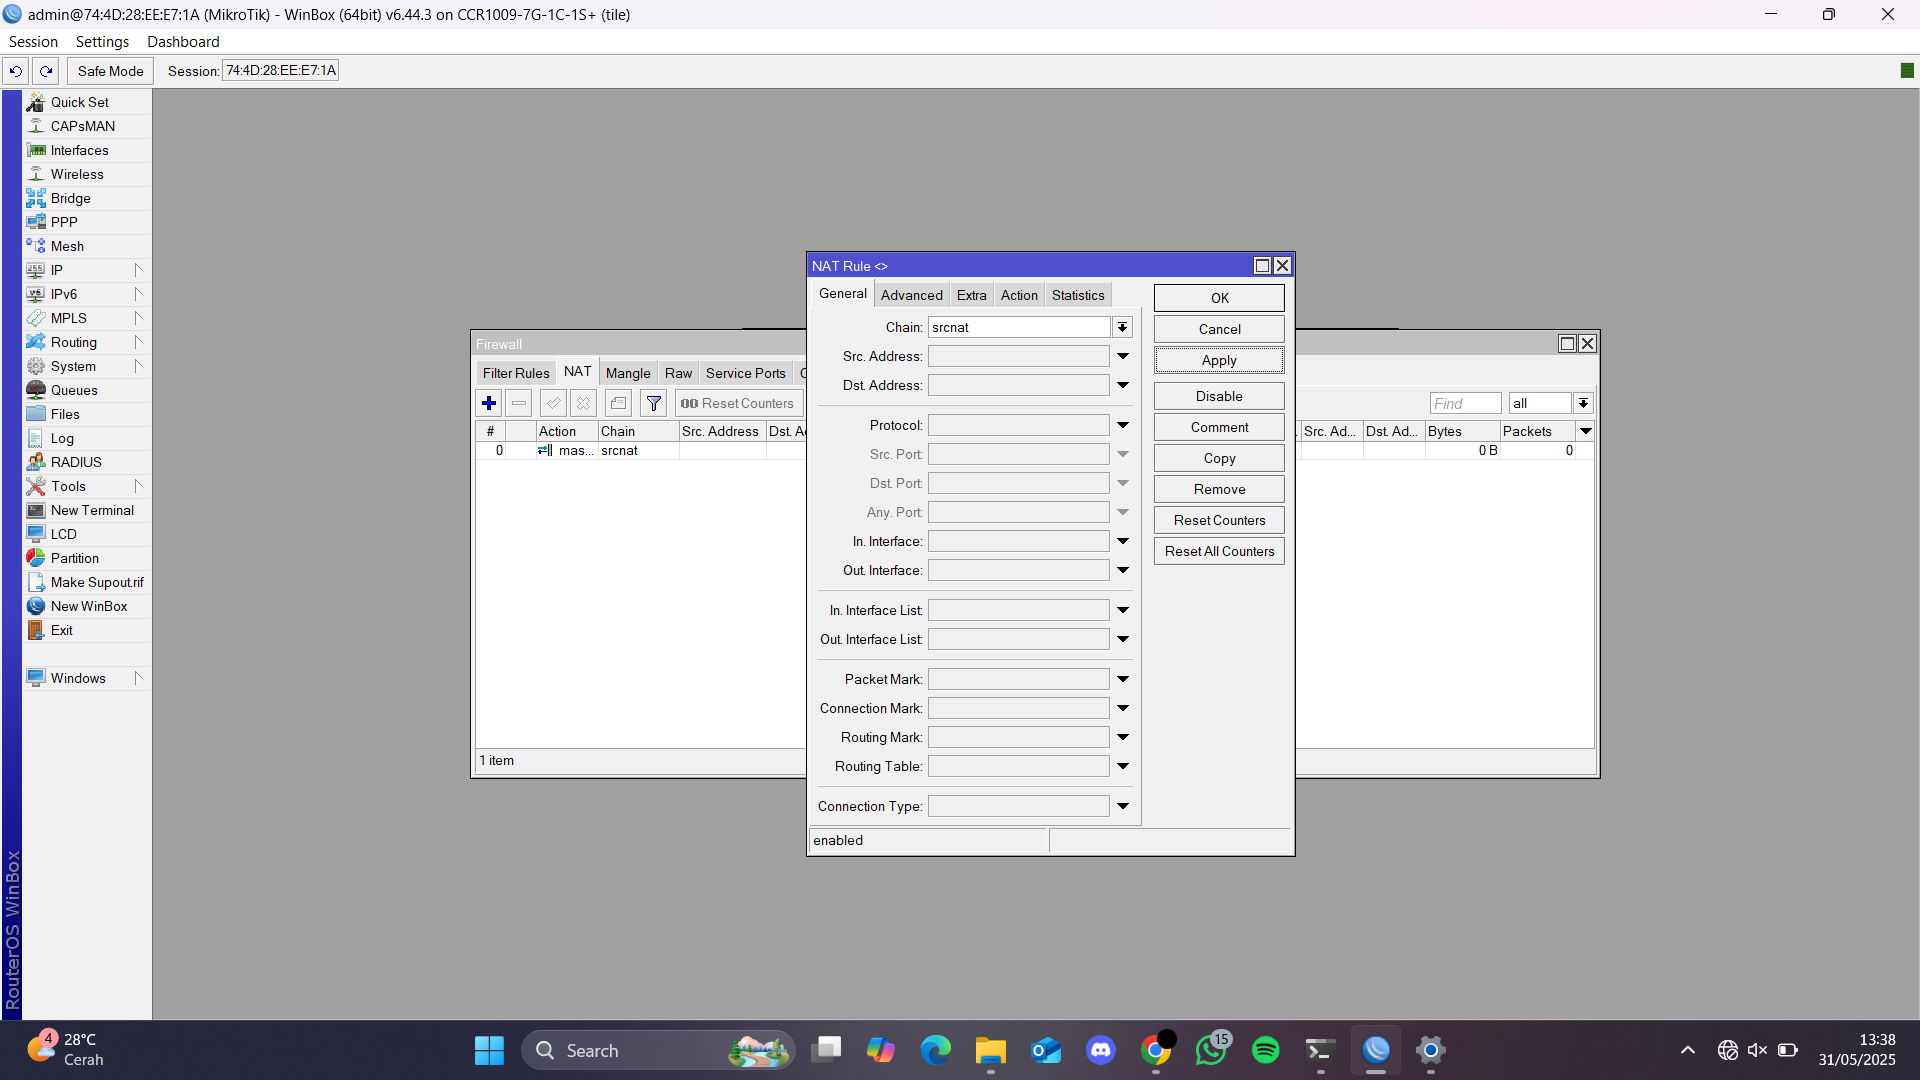
\includegraphics[width=\linewidth]{P4/img/nat (2).png}
			\caption{Konfigurasi chain\label{fig:konfigurasiR1}}
		\end{subfigure}
		\begin{subfigure}[b]{0.4\linewidth}
			\centering
			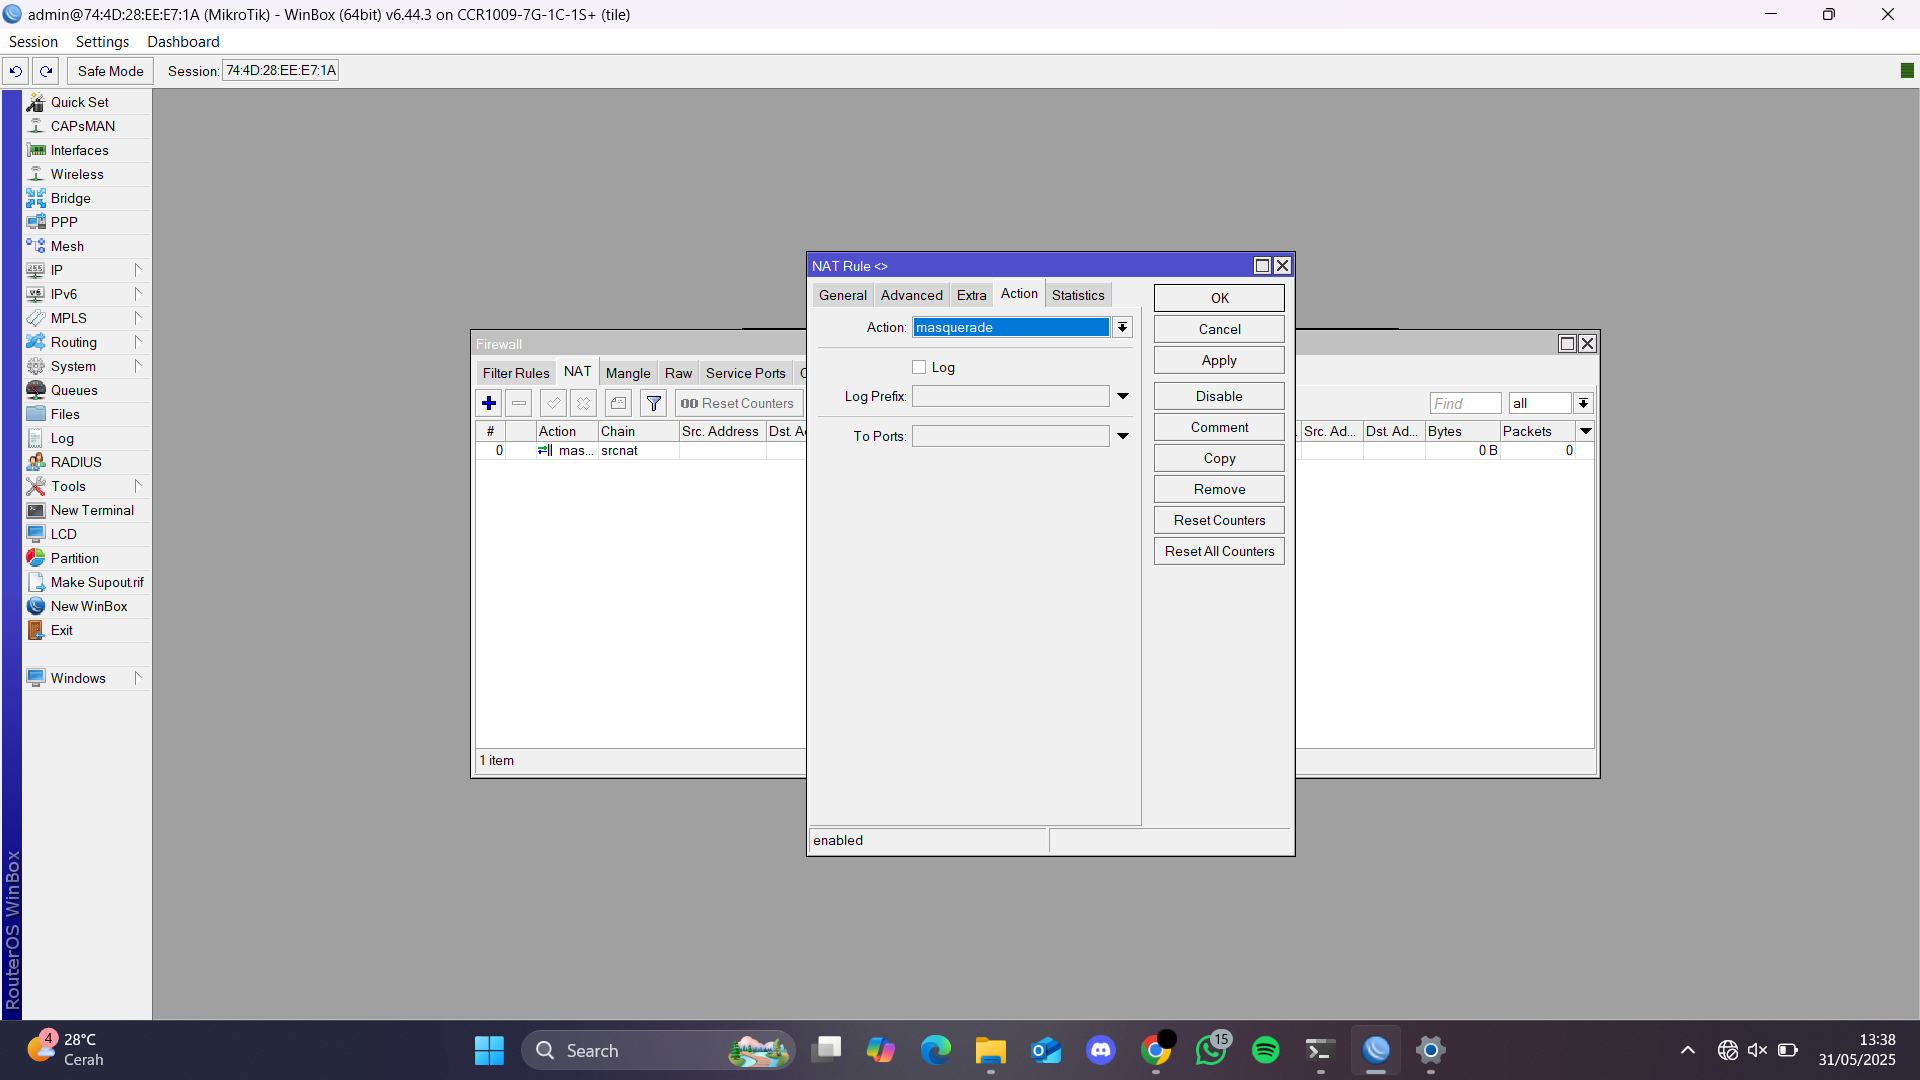
\includegraphics[width=\linewidth]{P4/img/nat (1).png}
			\caption{Konfigurasi action\label{fig:konfigurasiR2}}
		\end{subfigure}
		\caption{Konfigurasi NAT}
		\hspace{1cm}
	\end{figure}
	\item Menguji NAT dengan melakukan ping ke 8.8.8.8 dari router melalui interface winbox.
	\begin{figure}[H]
		\centering
		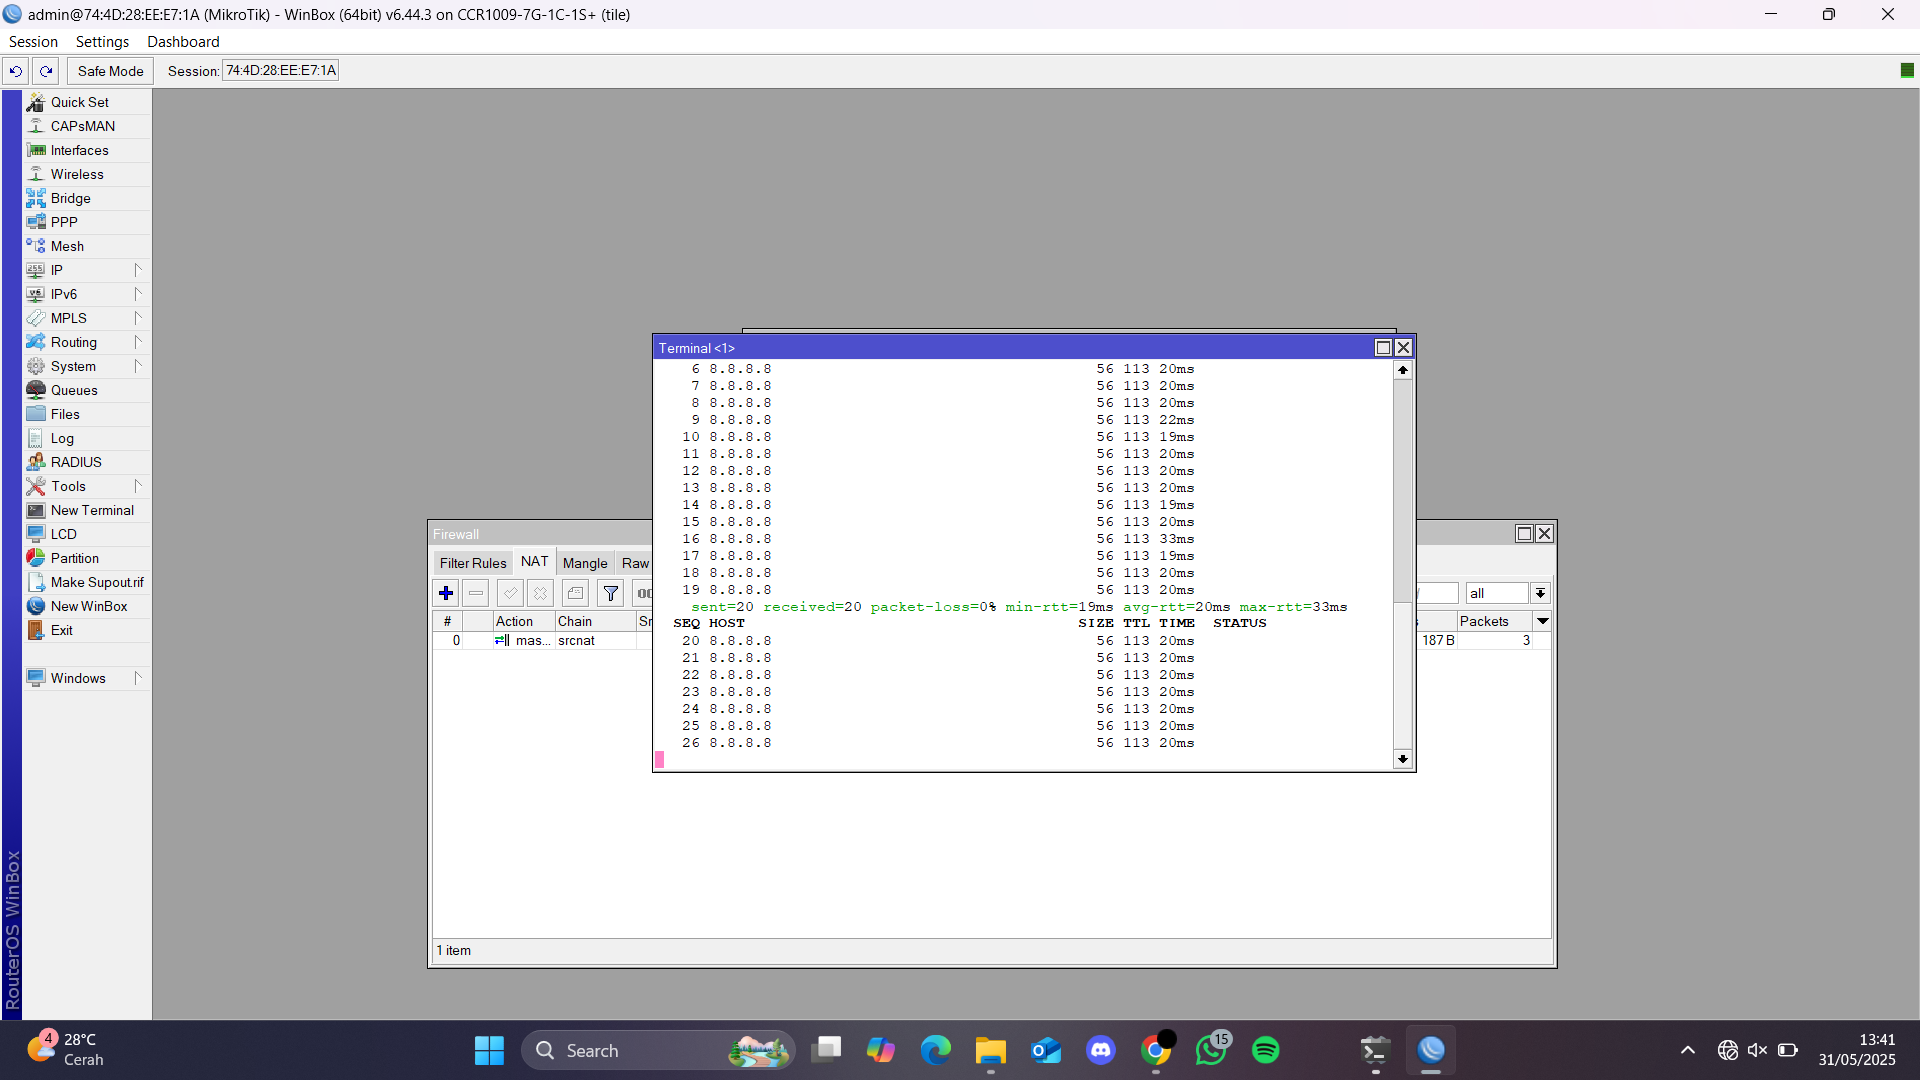
\includegraphics[width=\linewidth]{P4/img/ping 8888.png}
		\caption{Tes ping 8.8.8.8}
		\hspace{1cm}
	\end{figure}
	\item Melakukan konfigurasi firewall dengan menambahkan aturan baru untuk pemblokiran ICMP dan content blocking. Untuk aturan pemblokiran ICMP menggunakan konfigurasi Chain: forward, ProtocolL icmp, In.Interface: ether7, Action: drop. Untuk aturan pemblokiran konten menggunakan konfigurasi Chain: forward, Protocol: tcp, Dsr. Port: 80,443, In. Interface: ether7, Out. Interface: ether1, Content: speedtest, Action: drop.
	\begin{figure}[H]
		\centering
		\begin{subfigure}[b]{0.4\linewidth}
			\centering
			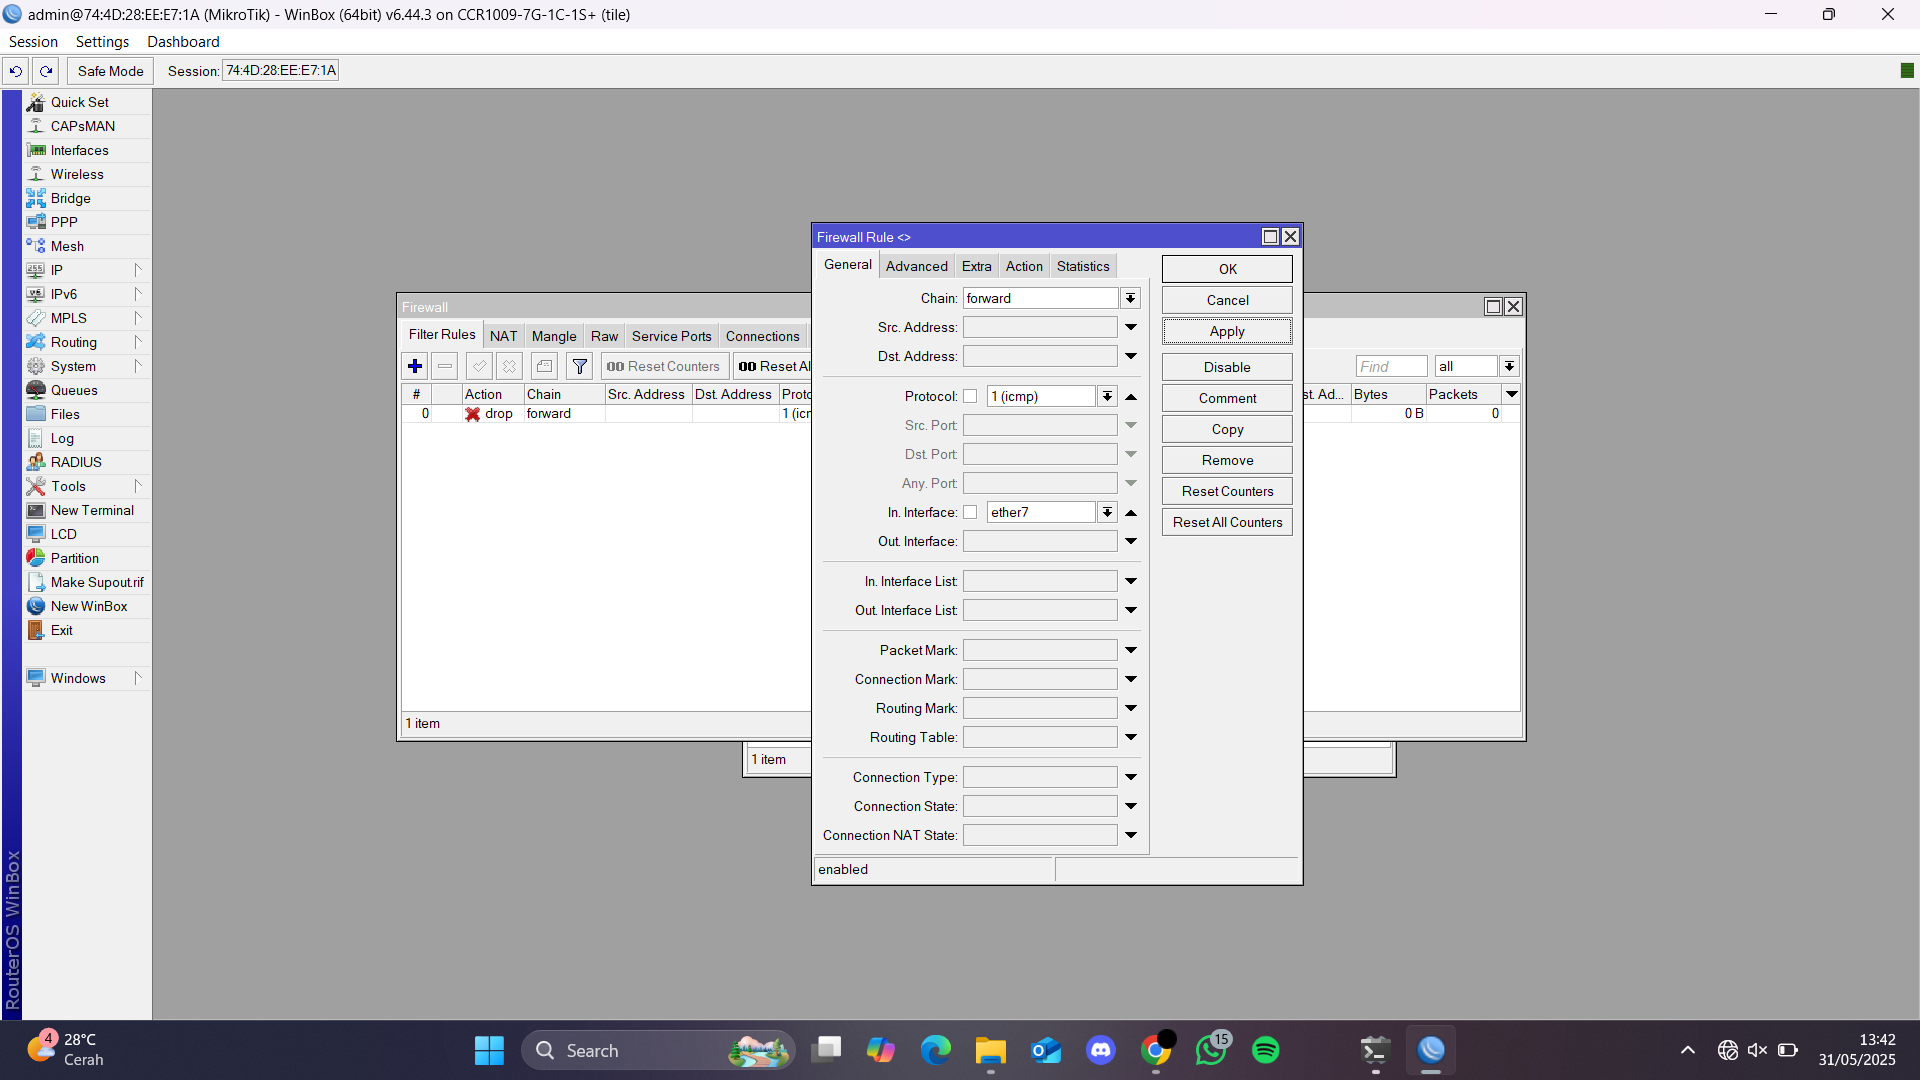
\includegraphics[width=\linewidth]{P4/img/firewall (2).png}
			\caption{Konfigurasi ICMP\label{fig:konfigurasiR1}}
		\end{subfigure}
		\begin{subfigure}[b]{0.4\linewidth}
			\centering
			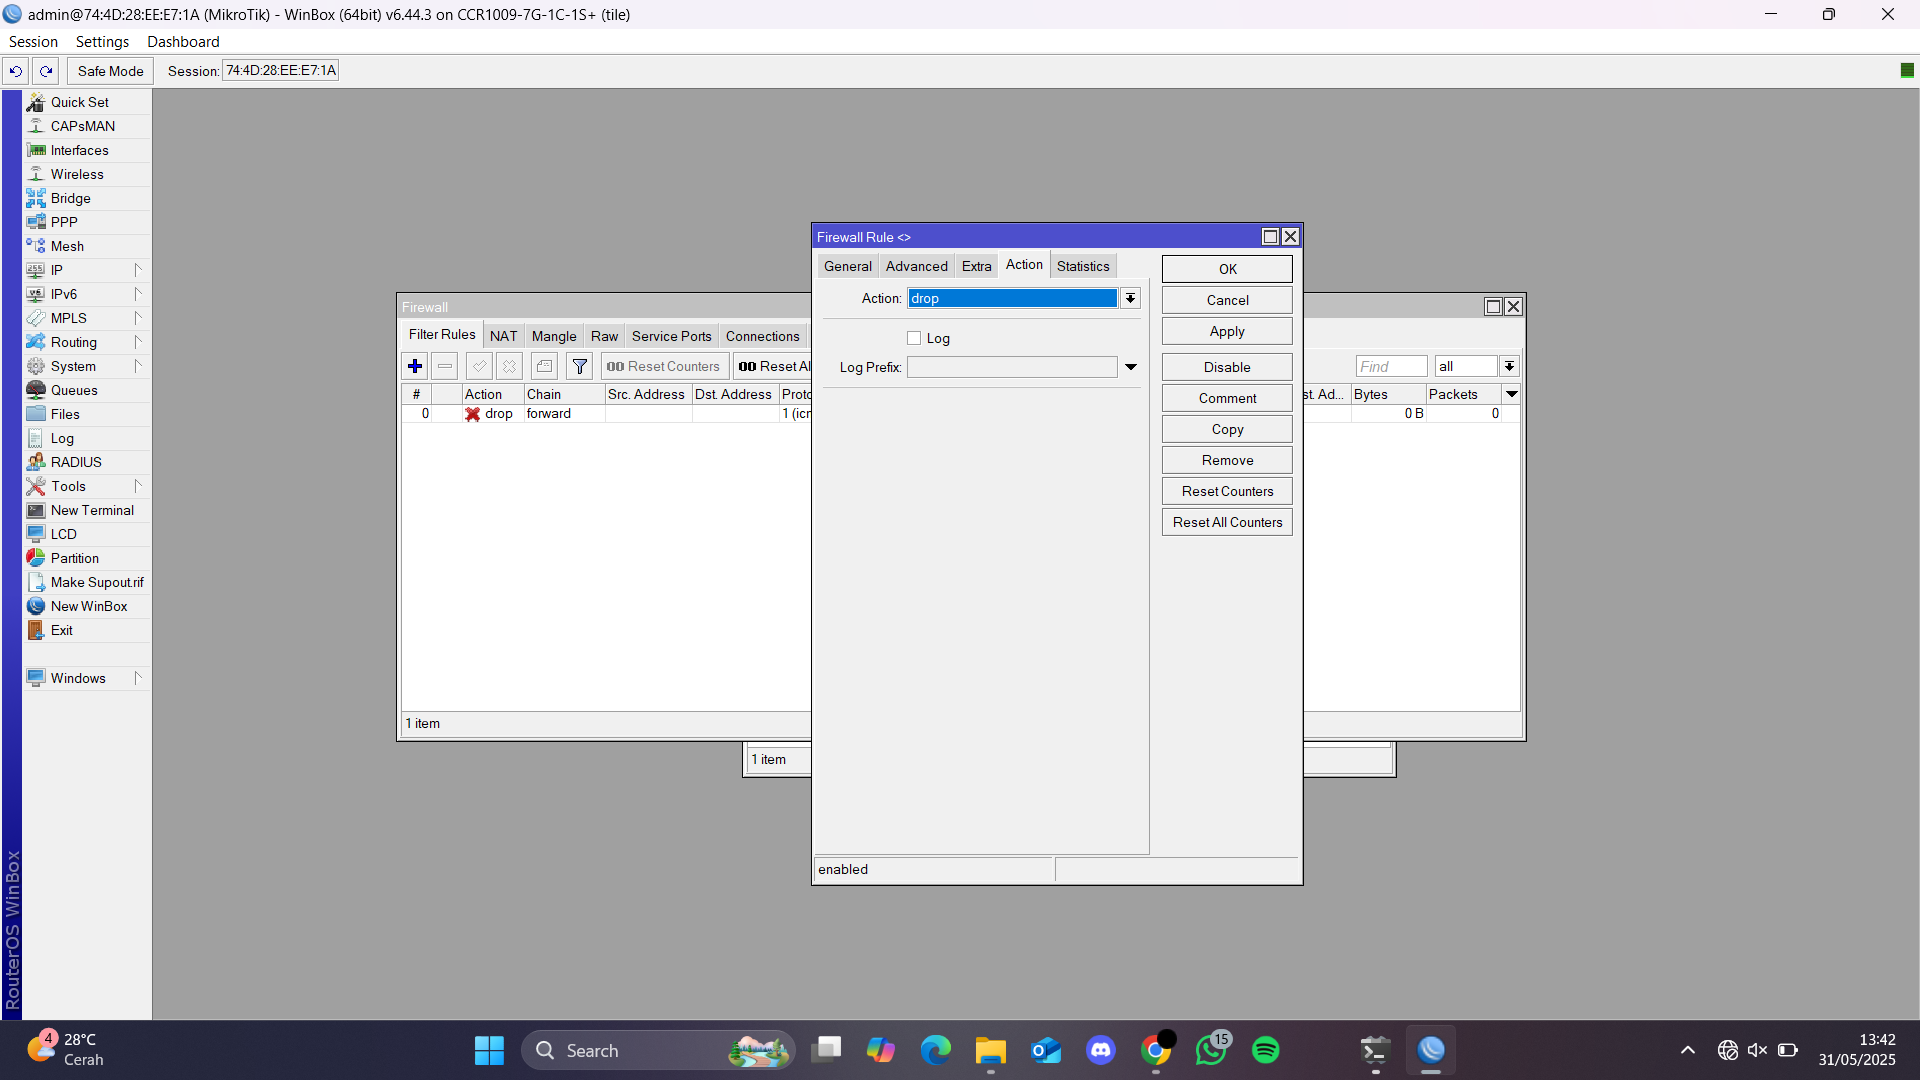
\includegraphics[width=\linewidth]{P4/img/firewall (3).png}
			\caption{Konfigurasi action ICMP\label{fig:konfigurasiR2}}
		\end{subfigure}
		\begin{subfigure}[b]{0.4\linewidth}
			\centering
			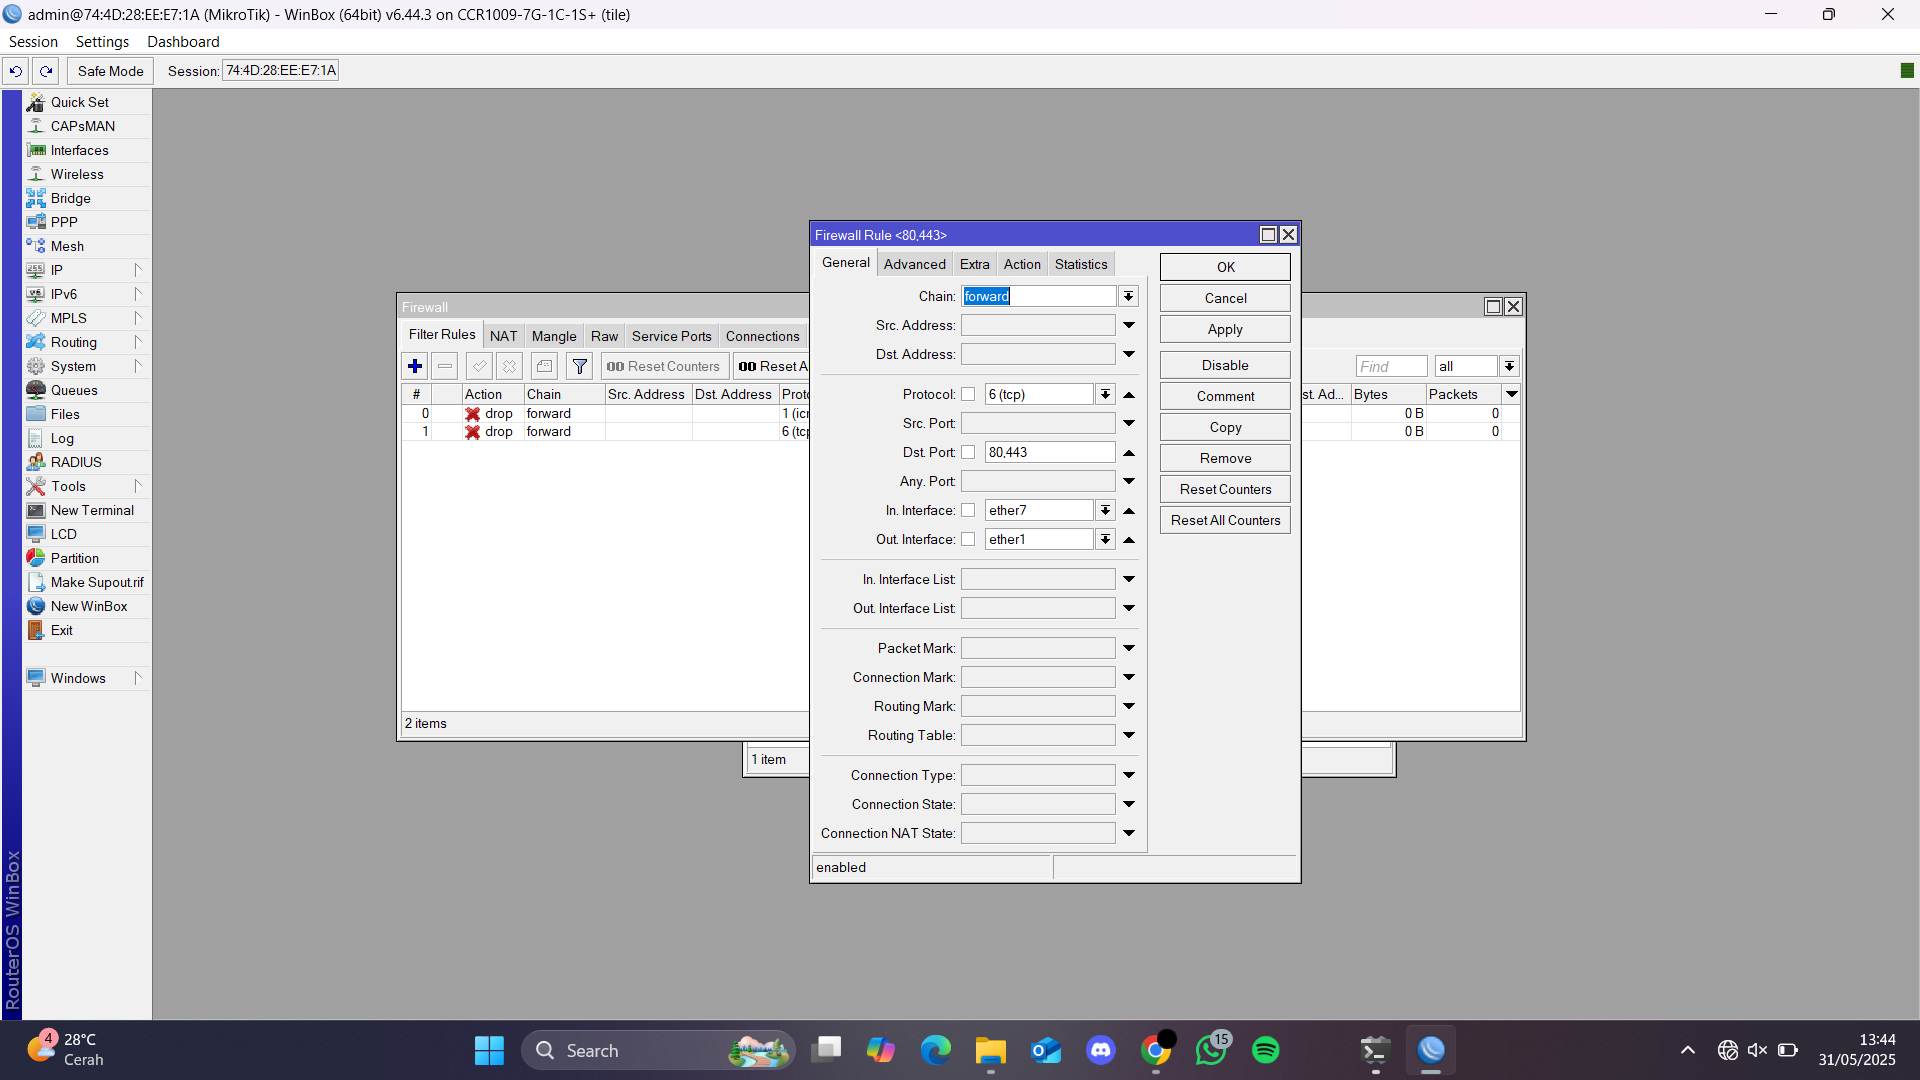
\includegraphics[width=\linewidth]{P4/img/firewall (4).png}
			\caption{Konfigurasi content block\label{fig:konfigurasiR1}}
		\end{subfigure}
		\begin{subfigure}[b]{0.4\linewidth}
			\centering
			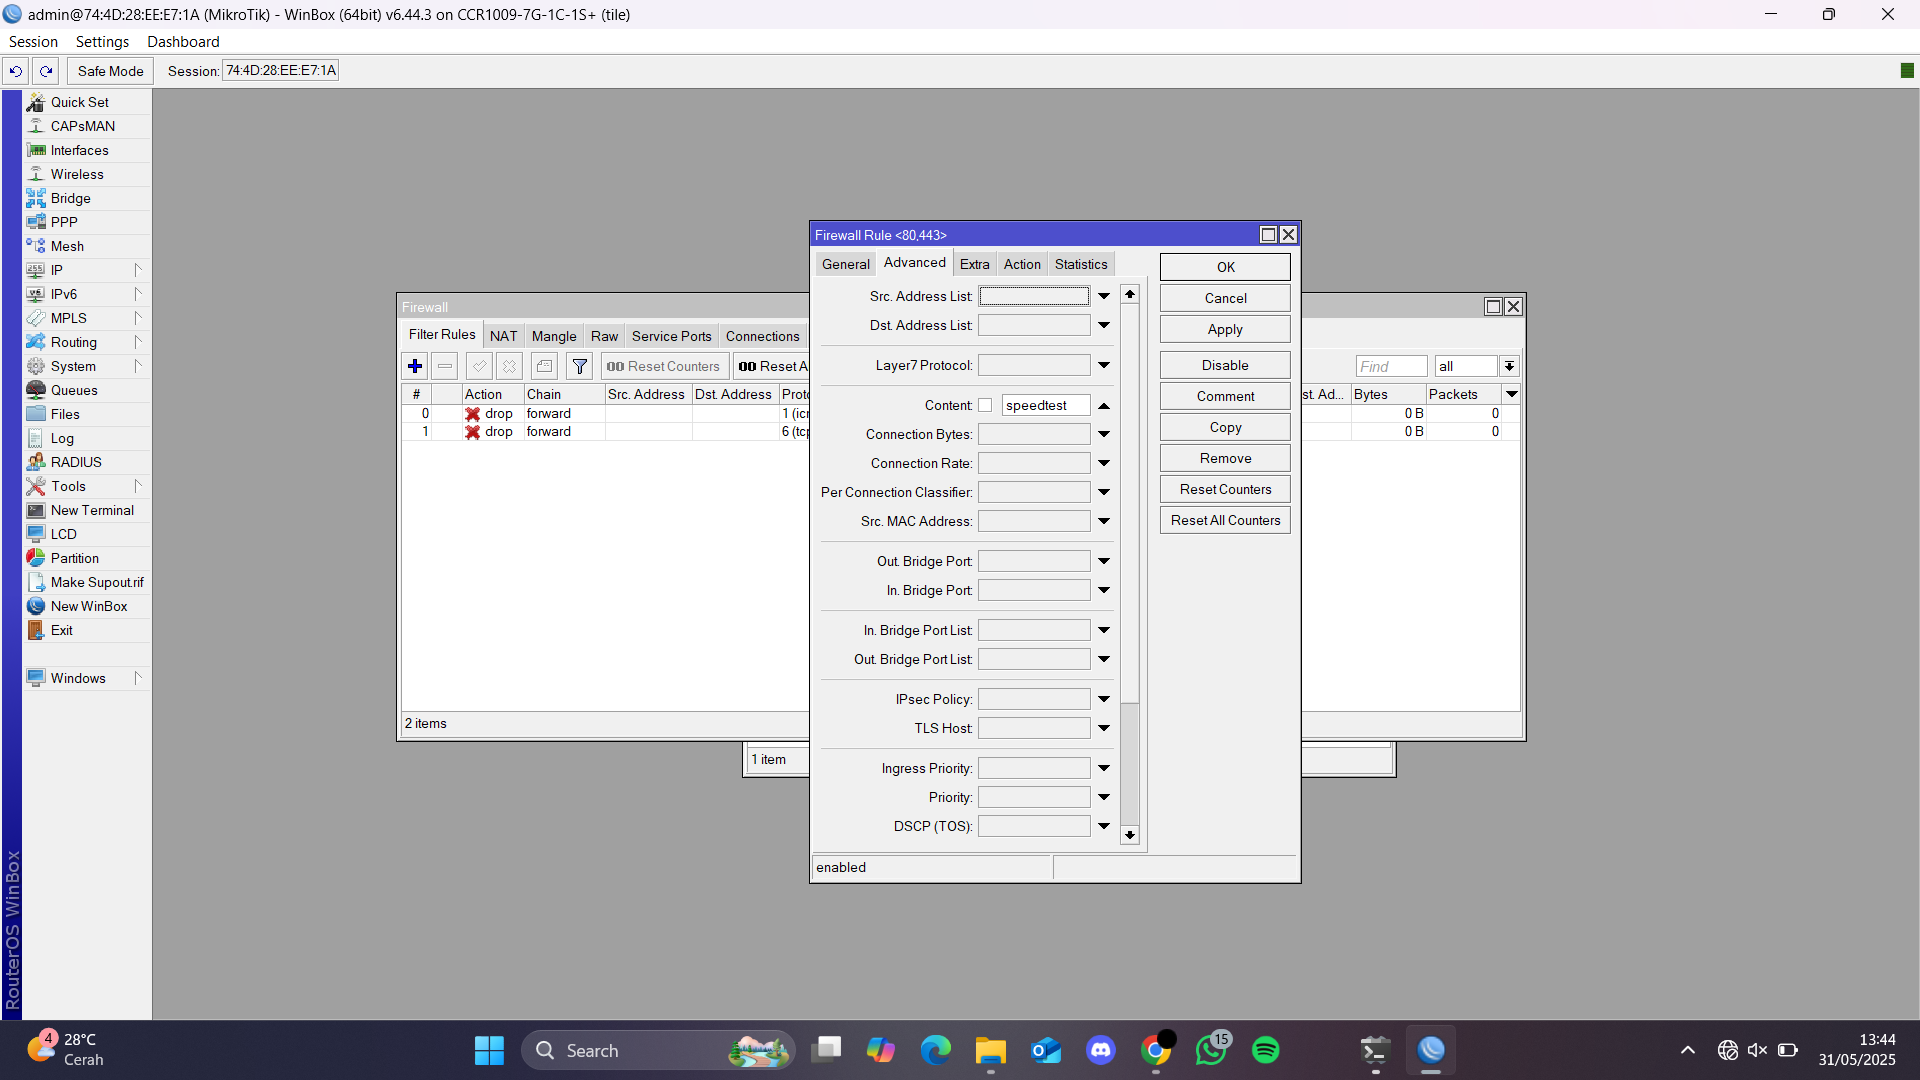
\includegraphics[width=\linewidth]{P4/img/firewall (5).png}
			\caption{Konfigurasi keyword content block\label{fig:konfigurasiR2}}
		\end{subfigure}
		\begin{subfigure}[b]{0.4\linewidth}
			\centering
			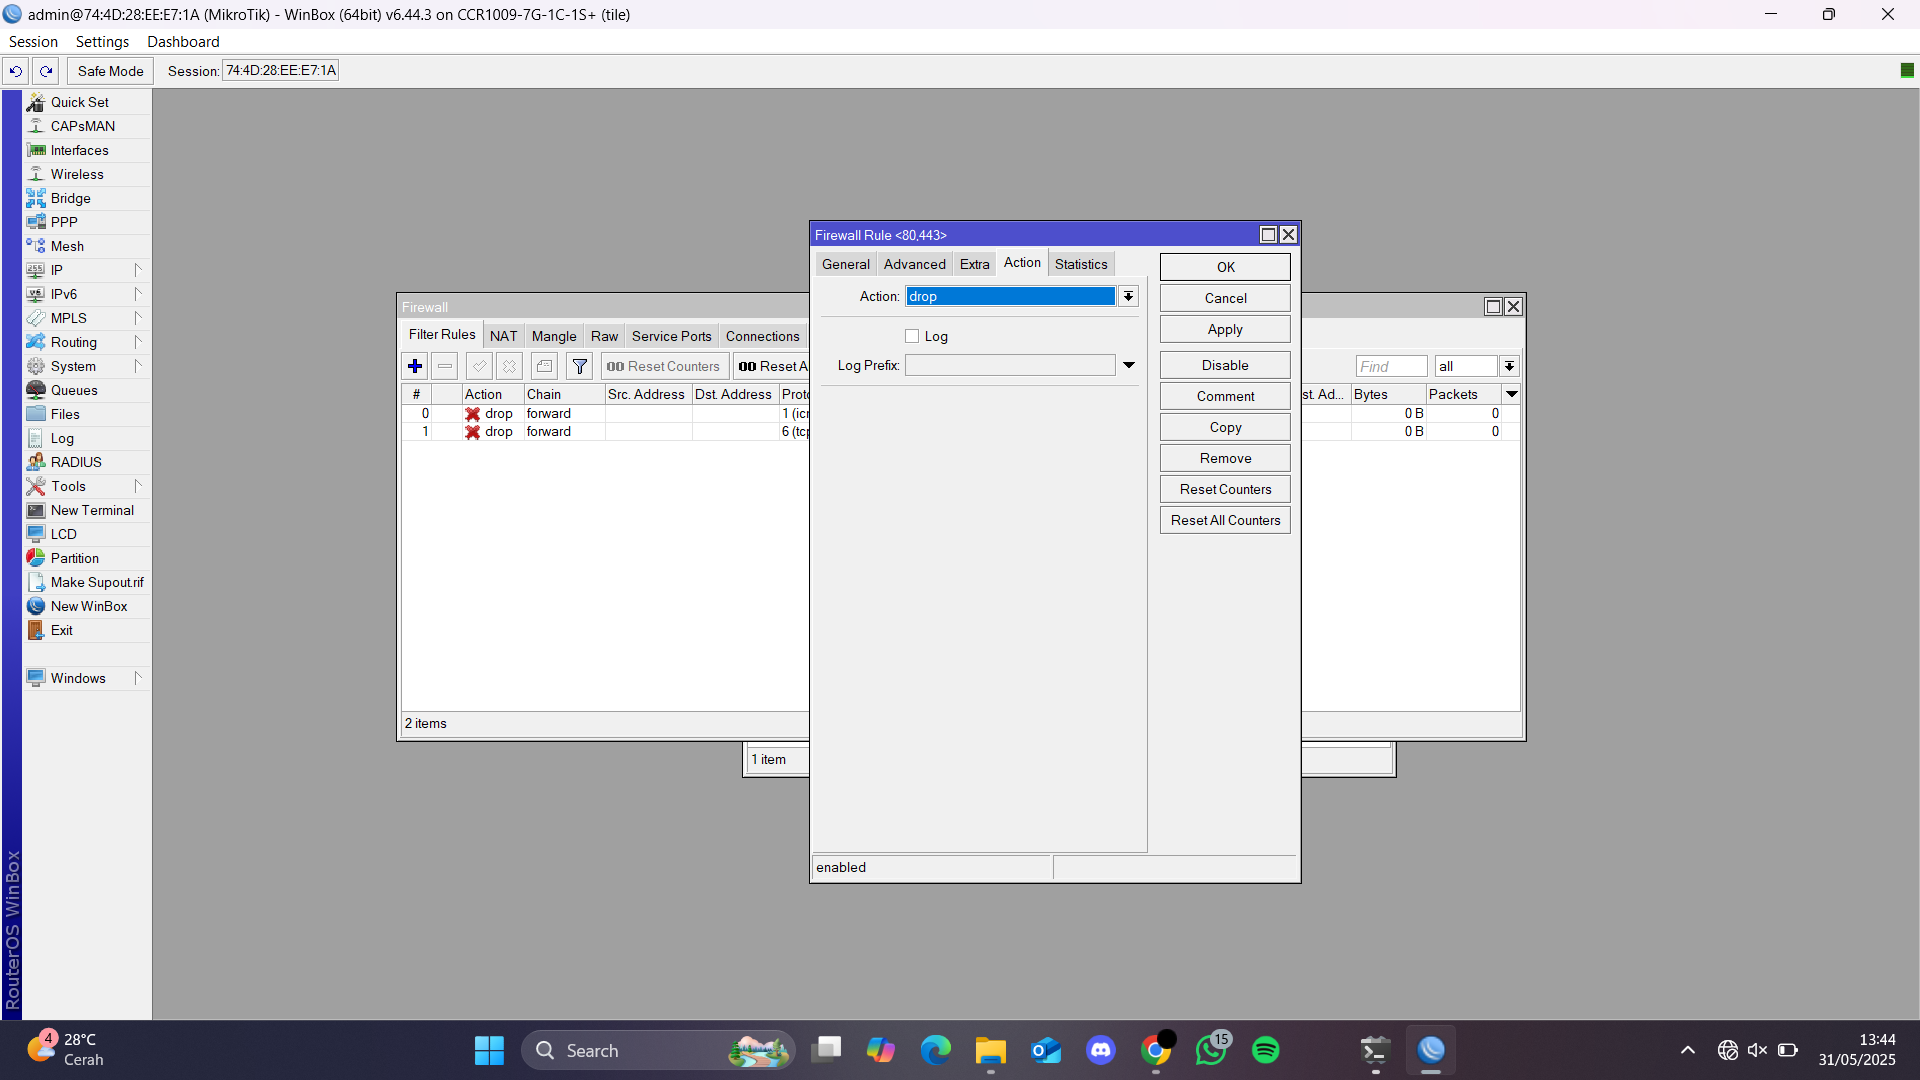
\includegraphics[width=\linewidth]{P4/img/firewall (1).png}
			\caption{Konfigurasi action content block\label{fig:konfigurasiR2}}
		\end{subfigure}
		\caption{Konfigurasi Firewall}
		\hspace{1cm}
	\end{figure}
	\item Melakukan konfigurasi bridge pada router B dengan menambahkan bridge baru dengan konfigurasi port yang digunakan adalah interface yang terhubung pada laptop dan interface yang terhubung dengan router A.
	\begin{figure}[H]
		\centering
		\begin{subfigure}[b]{0.4\linewidth}
			\centering
			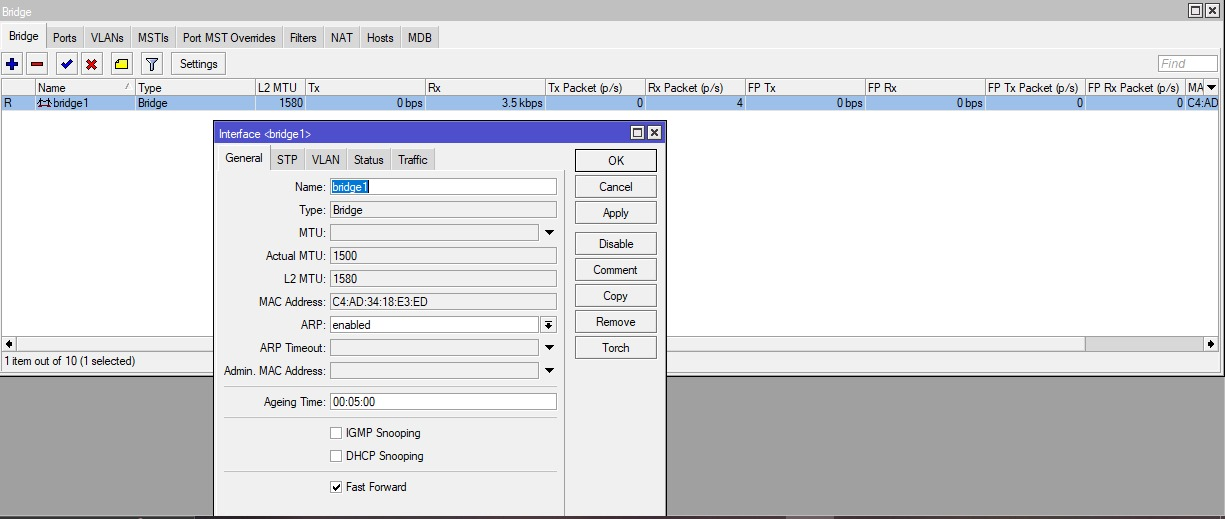
\includegraphics[width=\linewidth]{P4/img/bridge pre.jpg}
			\caption{Menambahkan bridge\label{fig:konfigurasiR1}}
		\end{subfigure}
		\begin{subfigure}[b]{0.4\linewidth}
			\centering
			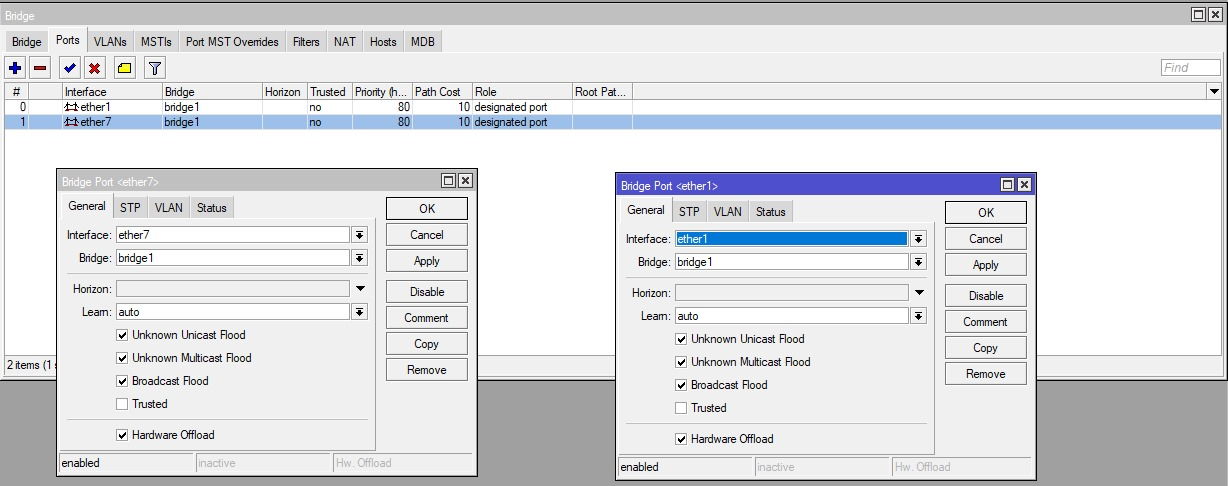
\includegraphics[width=\linewidth]{P4/img/bridge.jpg}
			\caption{Pengaturan port bridge\label{fig:konfigurasiR2}}
		\end{subfigure}
		\caption{Konfigurasi bridge router B}
		\hspace{1cm}
	\end{figure}
	\item Melakukan konfigurasi IP pada laptop. Karena IP diberikan secara otomatis oleh server DHCP, maka hanya perlu memeriksa IP yang diberikan oleh server melalui command ipconfig pada cmd atau powershell.
	\item Menguji aturan ICMP dengan melakukan ping ke 8.8.8.8 dengan keadaan firewall aktif dan nonaktfi.
	\item Menguji aturan content blocking dengan mengakses speedtest.net dengan keadaan firewall aktif dan nonaktif.
\end{enumerate}
\section{Analisis Hasil Percobaan}
Pada praktikum ini dilakukan percobaan pengaturan firewall dan NAT pada router mikrotik. Secara teori, bila konfigurasi NAT berhasil maka router dapat melakukan ping ke 8.8.8.8 dan mendapat balasan. Bila konfigurasi firewall berhasil, maka bila aturan pemblokiran ICMP diaktifkan maka laptop bisa melakukan ping ke 8.8.8.8 tapi tidak akan mendapat jawaban (time out) dan bila aturan pemblokiran konten diaktifkan maka laptop tidak akan bisa membuka konten dari situs web yang mengandung kata kunci "speedtest" dan akan diberi message time out oleh browser. Setelah percobaan dilakukan, didapatkan hasil bahwa router A dapat melakukan ping 8.8.8.8, yang artinya pengaturan NAT sudah berhasil. Saat firewall aturan pemblokiran ICMP diaktifkan, laptop tidak bisa mendapatkan respon time out ketika melakukan ping ke 8.8.8.8 dan baru bisa mendapat balasan apabila aturan firewall untuk pemblokiran ICMP dimatikan. Hal ini menunjukkan bahwa pemblokiran ICMP ke alamat 8.8.8.8 dengan action drop telah berhasil karena laptop dapat melakukan ping namun tidak mendapat balasan (drop) saat aturan firewall aktif.\begin{figure}[H]
	\centering
		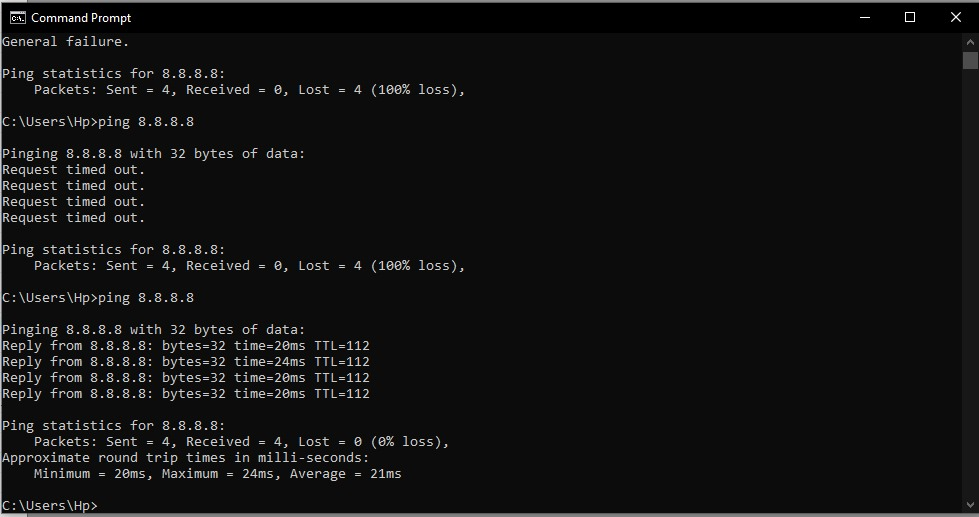
\includegraphics[width=\linewidth]{P4/img/ping fw off.jpg}
		\caption{Hasil ping 8.8.8.8 dari laptop. Bagian atas adalah saat firewall dinyalakan dan bagian bawah adalah saat firewall dimatikan\label{fig:konfigurasiR1}}
\end{figure}
Saat firewall aturan pemblokiran konten diaktifkan, laptop tidak bisa membuka situs speedtest.net melalui browser dan muncul peringatan connection timed out dan baru bisa mengakses kembali situs speedtest.net ketika aturan firewall dimatikan. Hal ini menunujukkan bahwa firewall aturan pemblokiran konten telah berhasil memblokir akses laptop ke situs yang memiliki kata kunci "speedtest".
\begin{figure}[H]
	\centering
	\begin{subfigure}[b]{0.4\linewidth}
		\centering
		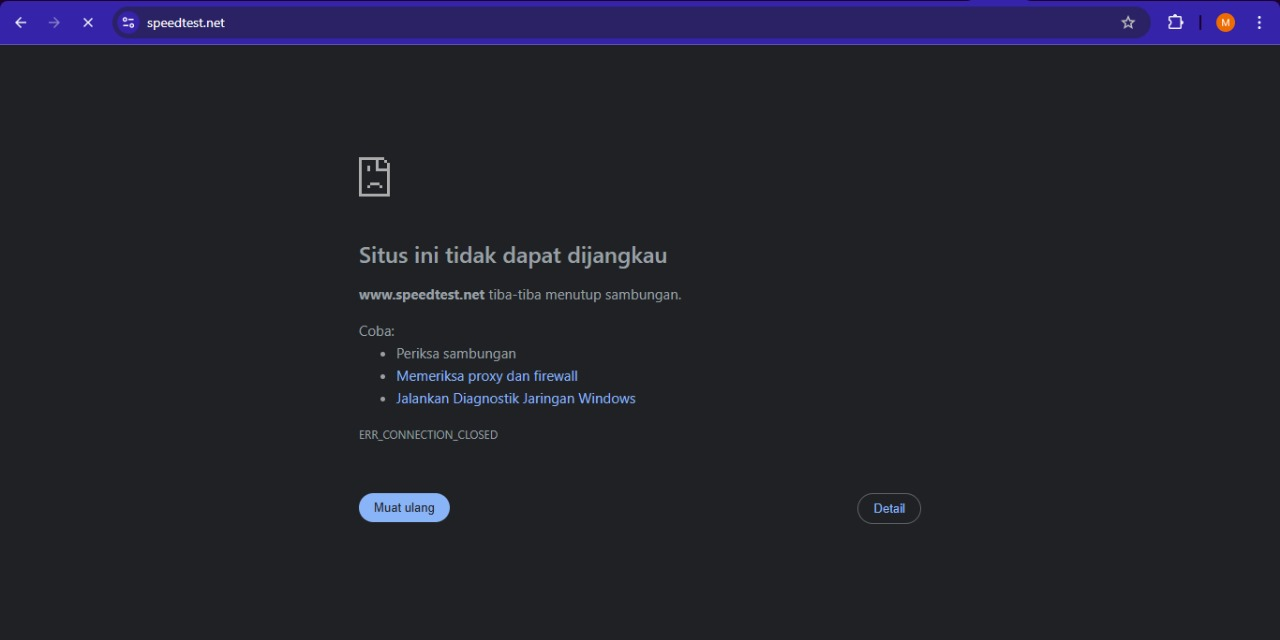
\includegraphics[width=\linewidth]{P4/img/speedtest fw in.jpg}
		\caption{Akses speedtest.net saat firewall aktif\label{fig:konfigurasiR1}}
	\end{subfigure}
	\begin{subfigure}[b]{0.4\linewidth}
		\centering
		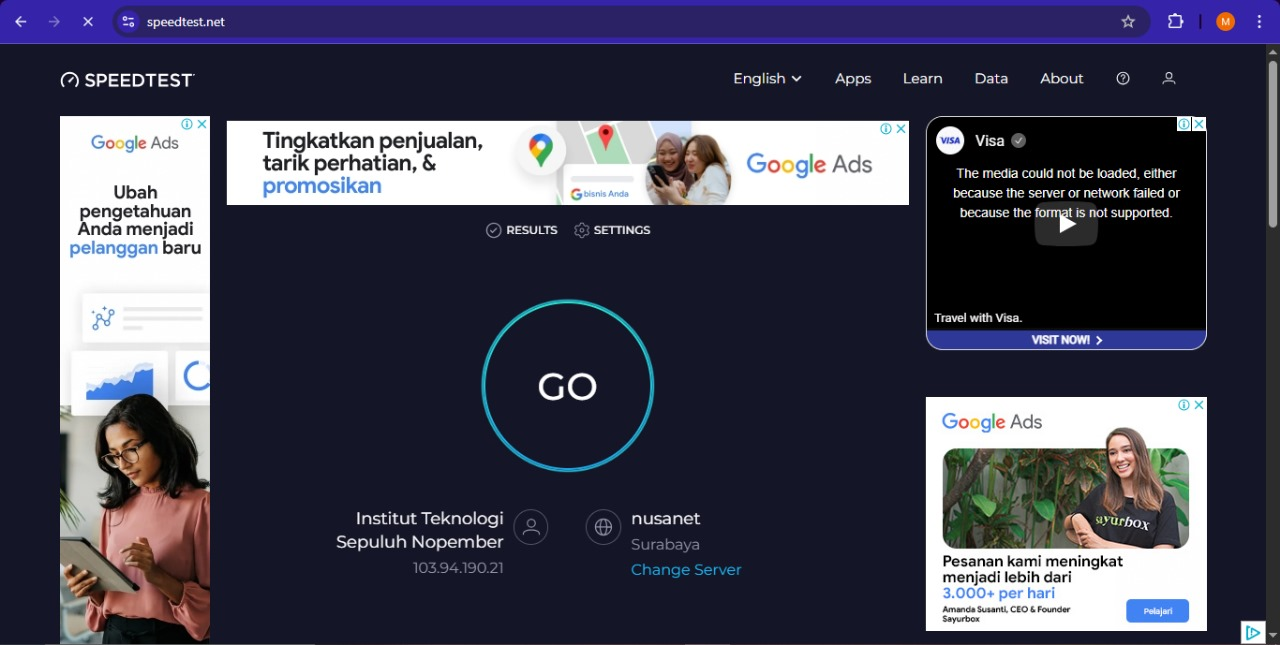
\includegraphics[width=\linewidth]{P4/img/speedtest fw off.jpg}
		\caption{Akses speedtest.net saat firewall mati\label{fig:konfigurasiR2}}
	\end{subfigure}
	\caption{Hasil akses speedtest.net}
	\hspace{1cm}
\end{figure}

\section{Hasil Tugas Modul}
Pada tugas modul ini, digunakan 1 server dengan IP lokal 192.168.105.1 dan IP publik 10.10.10.1, 1 router, 1 switch, dan 3 PC dengan IP address lokal masing masing 192.168.10.2, 192.168.10.3, 192.168.10.4. Interface fa0/0 router terhubung pada sercer dan fa1/0 terhubung pada switch. Berikut merupakan topologi jaringan:
\begin{figure}[H]
	\centering
	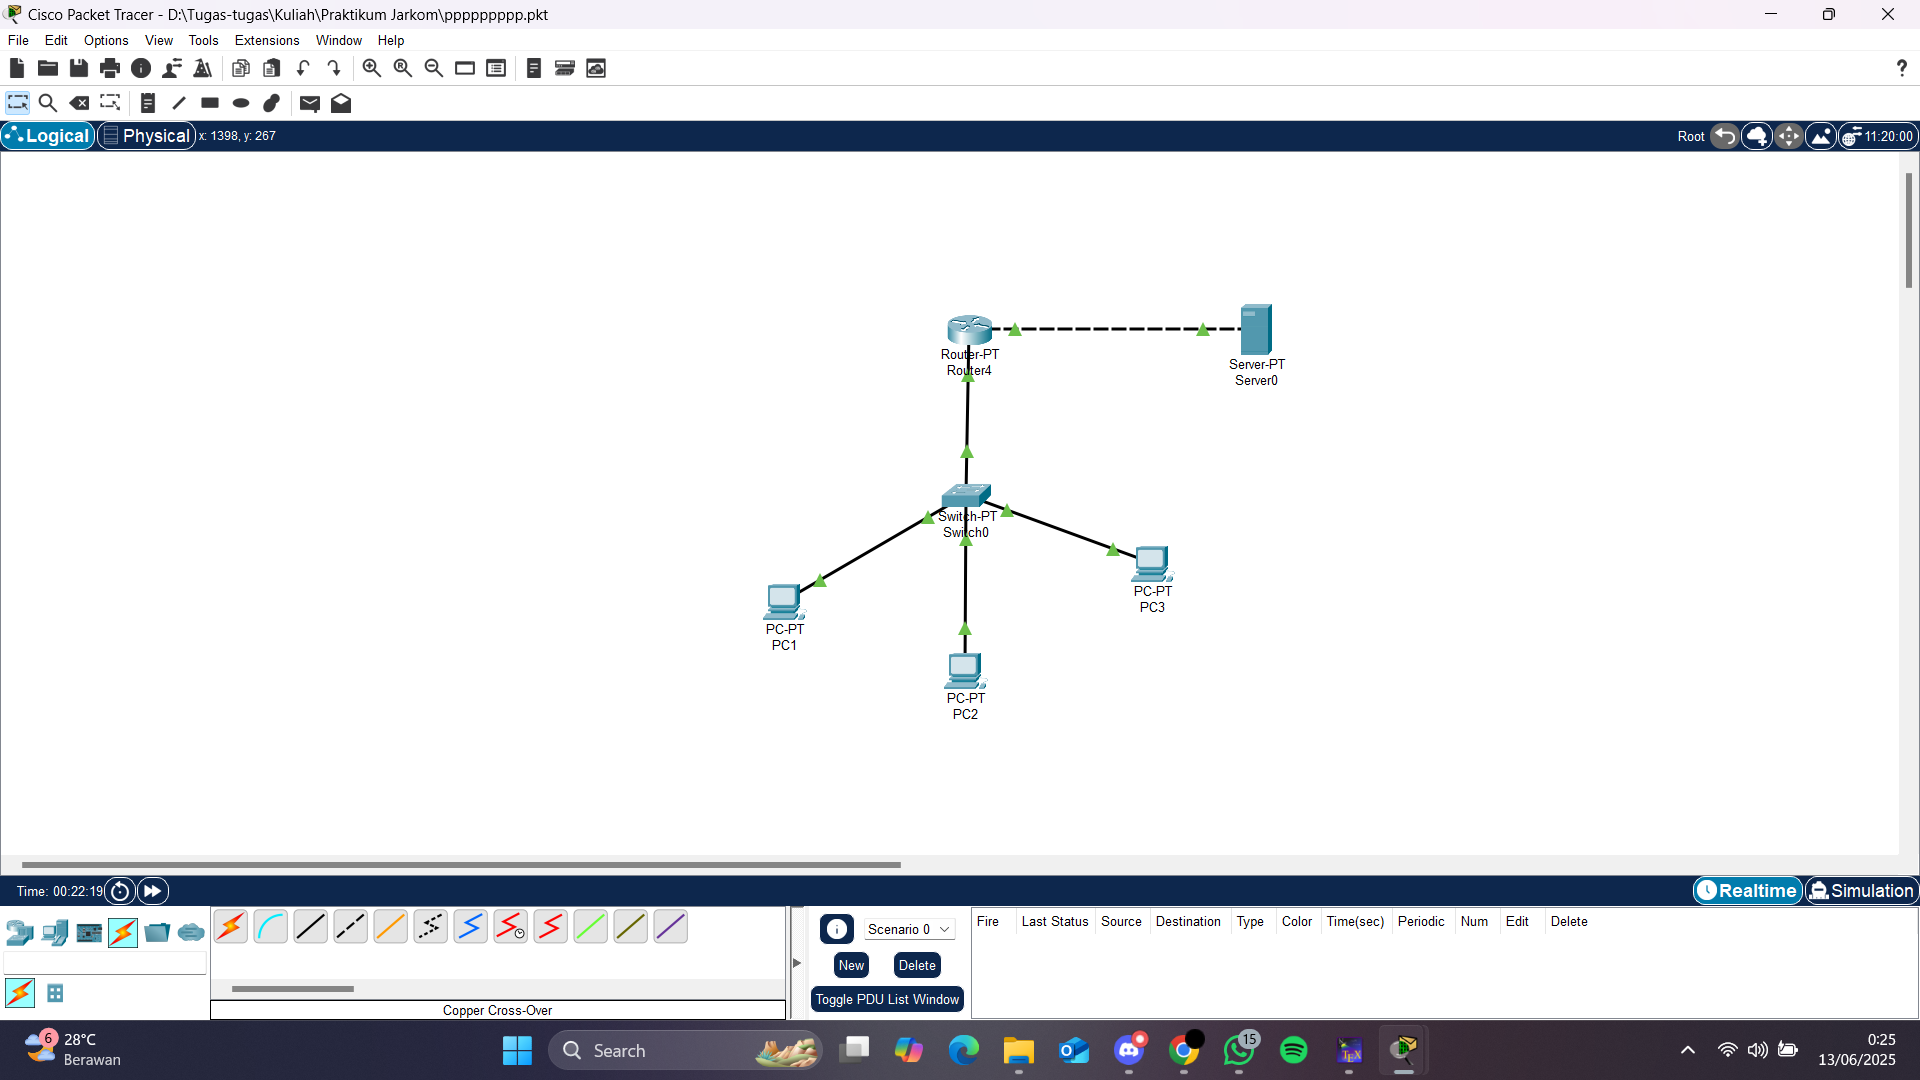
\includegraphics[width=\linewidth]{P4/img/tumod (6).png}
	\caption{Topolofi Tugas Modul}
	\hspace{1cm}
\end{figure}
untuk melakukan konfigurasi NAT, digunakan command sebagai berikut pada router:
\begin{lstlisting}
	Router(config)#ip nat inside source static 192.168.105.1 10.10.10.1
	Router(config)#interface fa0/0
	Router(config-if)#ip nat inside
	Router(config)#interface fa1/0
	Router(config-if)#ip nat outside
\end{lstlisting}
Dengan konfigurasi seperti di atas, maka ketiga PC dapat mengakses server menggunakan alamat IP publiknya yaitu 10.10.10.1.
\begin{figure}[H]
	\centering
	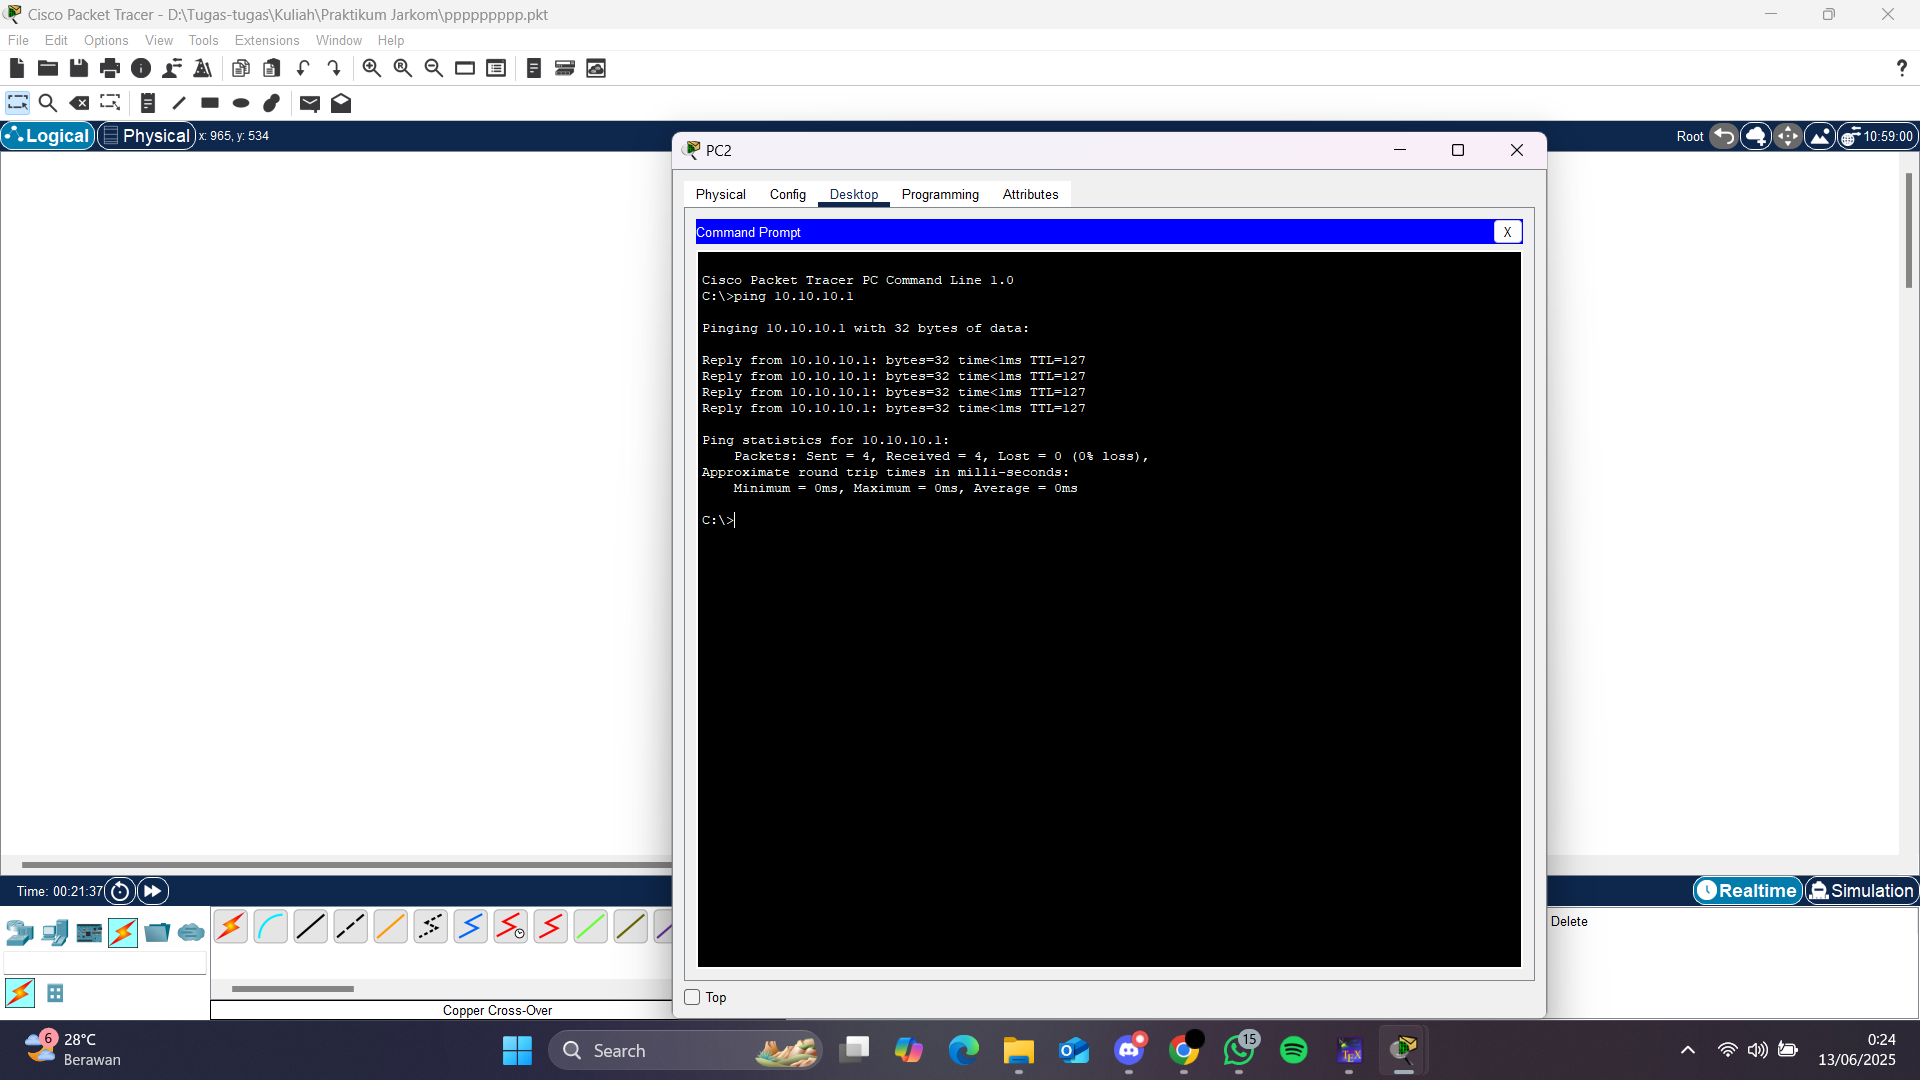
\includegraphics[width=\linewidth]{P4/img/tumod (4).png}
	\caption{Hasil ping server menggunakan IP publik dari PC2}
	\hspace{1cm}
\end{figure}
Penerapan firewall untuk memblokir masing-masing PC dapat diterapkan menggunakan command berikut:
\begin{lstlisting}
	Router(config)#access-list 100 deny icmp 192.168.10.3 0.0.0.0 192.168.105.0 0.0.0.0
	Router(config)#access-list 101 deny icmp 192.168.10.4 0.0.0.0 192.168.105.0 0.0.0.0
	Router(config)#access-list 102 deny icmp 192.168.10.2 0.0.0.0 192.168.105.0 0.0.0.0
\end{lstlisting}
Access list 100 digunakan untuk memblokir PC2, 101 digunakan untuk memblokir PC3, dan 102 dignakan untuk memblokir PC1. Untuk kasus pertama yaitu hanya PC1 yang bisa mengakses server maka PC2 dan PC3 harus diblokir. Pemblokiran diterapkan atau dinyalakan dengan command berikut:
\begin{lstlisting}
	Router(config)#interface fa1/0
	Router(config-if)#ip access-list 100 in
	Router(config-if)#ip access-list 101 in
	Router(config-if)#no ip access-list 102 in
\end{lstlisting}
Command di atas akan memblokir PC2 dan PC3 lalu mengangkat pemblokiran PC1, sehingga hanya PC1 yang bisa mengakses server. 
\begin{figure}[H]
	\centering
	\begin{subfigure}[b]{0.4\linewidth}
		\centering
		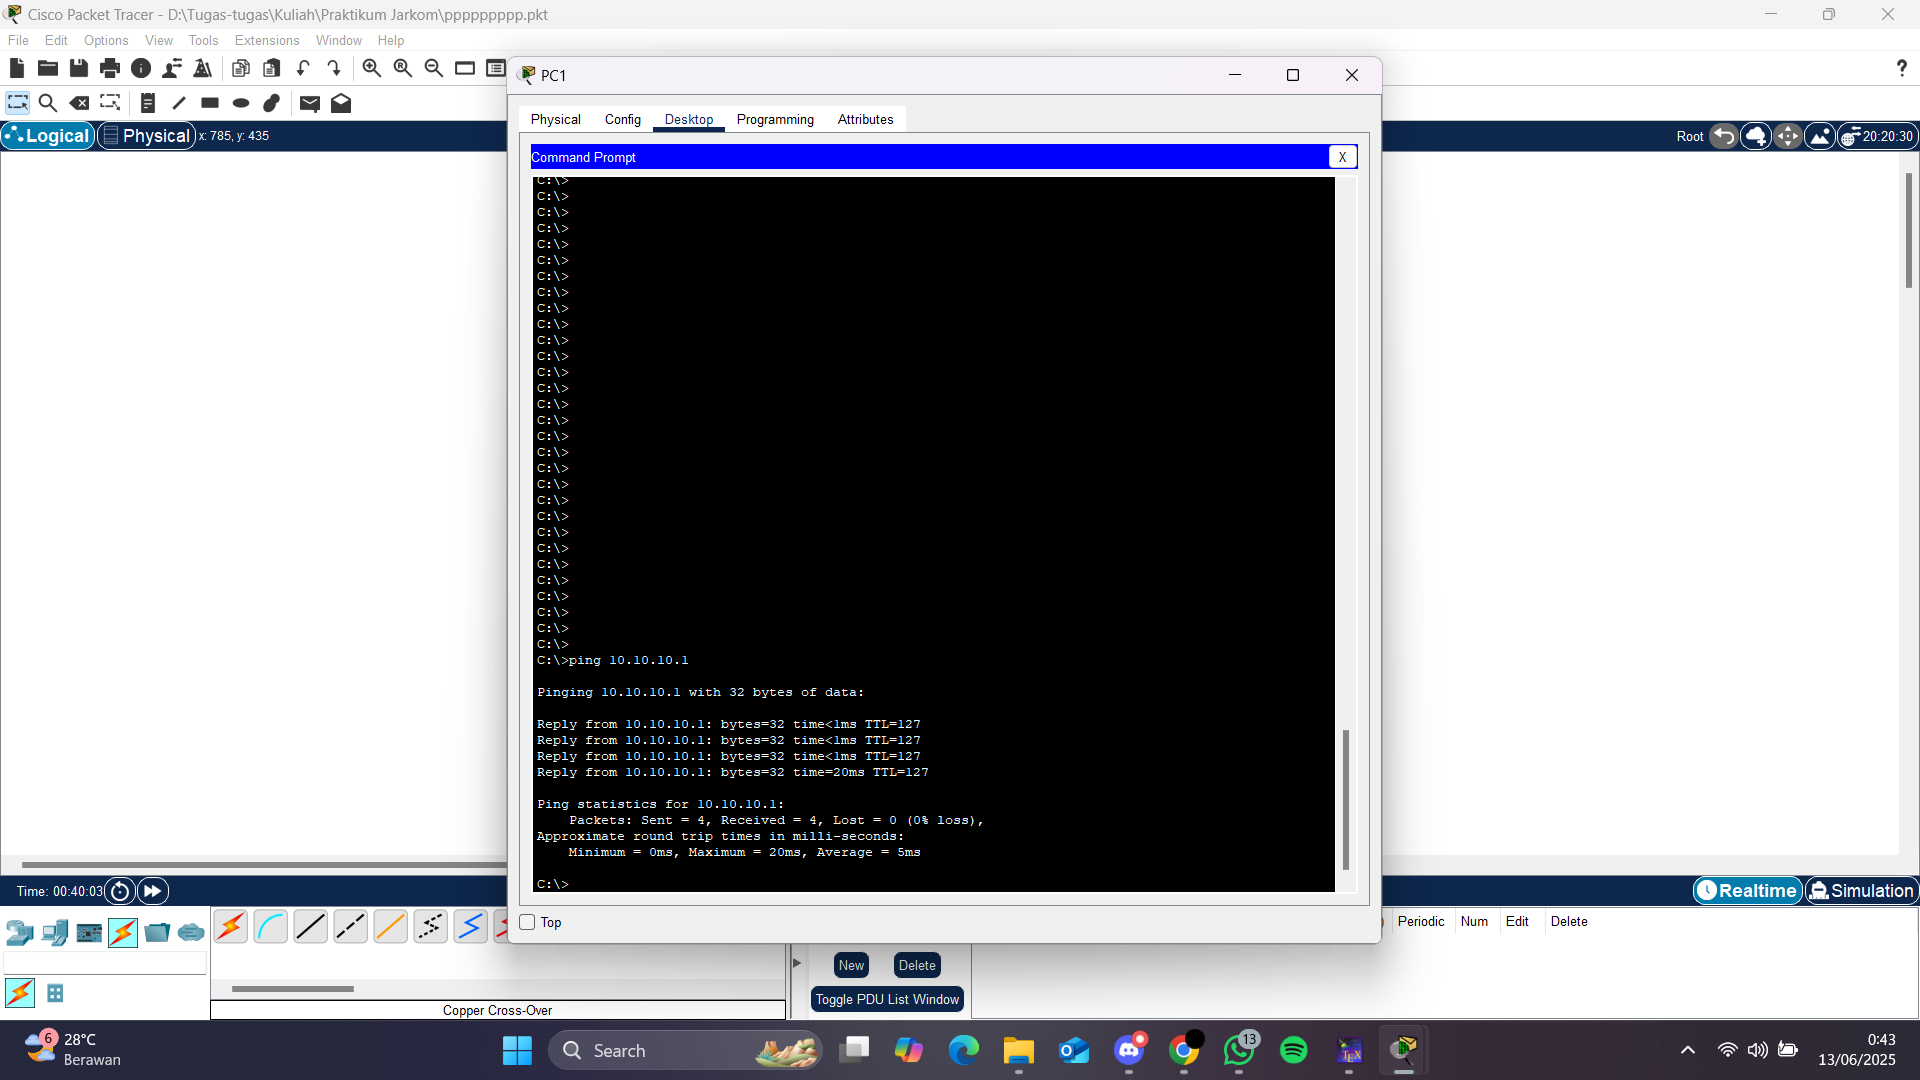
\includegraphics[width=\linewidth]{P4/img/tumod (10).png}
		\caption{Hasil ping ke server dari PC1\label{fig:konfigurasiR1}}
	\end{subfigure}
	\begin{subfigure}[b]{0.4\linewidth}
		\centering
		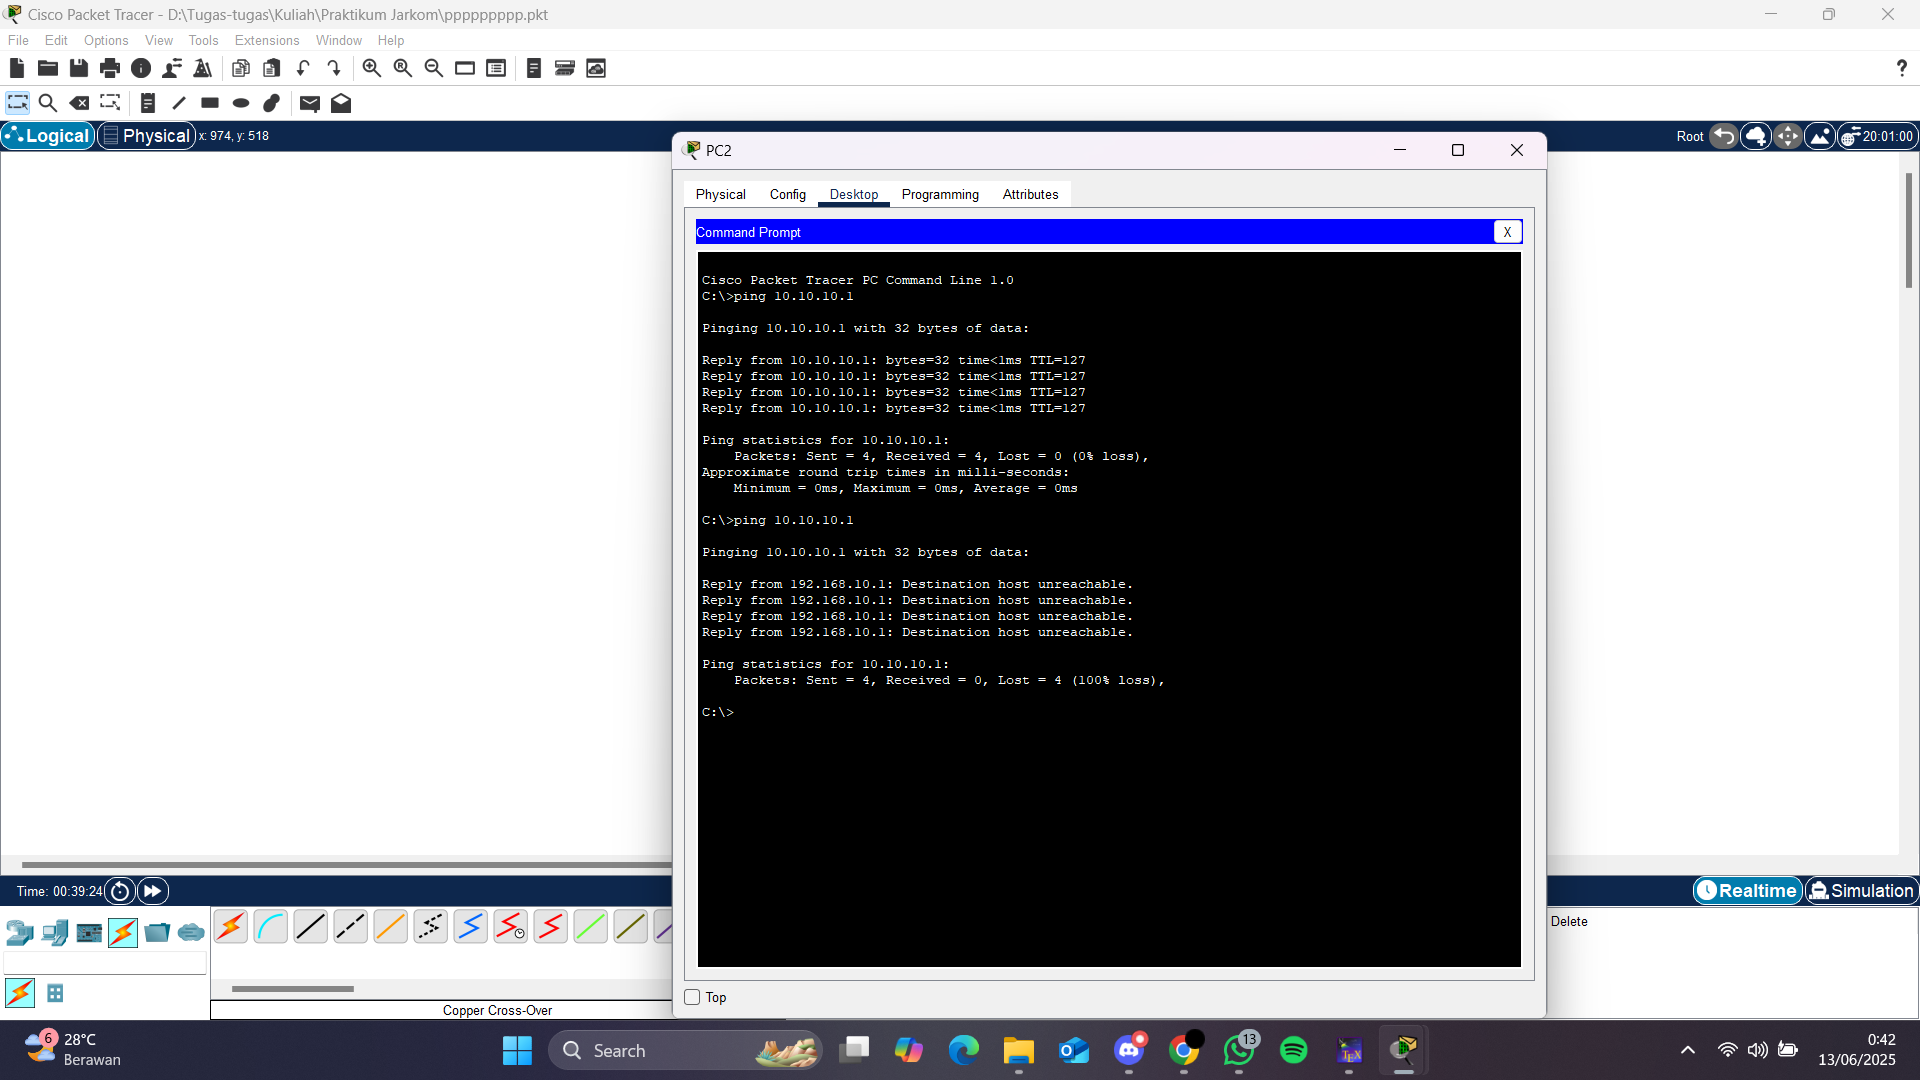
\includegraphics[width=\linewidth]{P4/img/tumod (9).png}
		\caption{Hasil ping ke server dari PC2\label{fig:konfigurasiR2}}
	\end{subfigure}
	\begin{subfigure}[b]{0.4\linewidth}
		\centering
		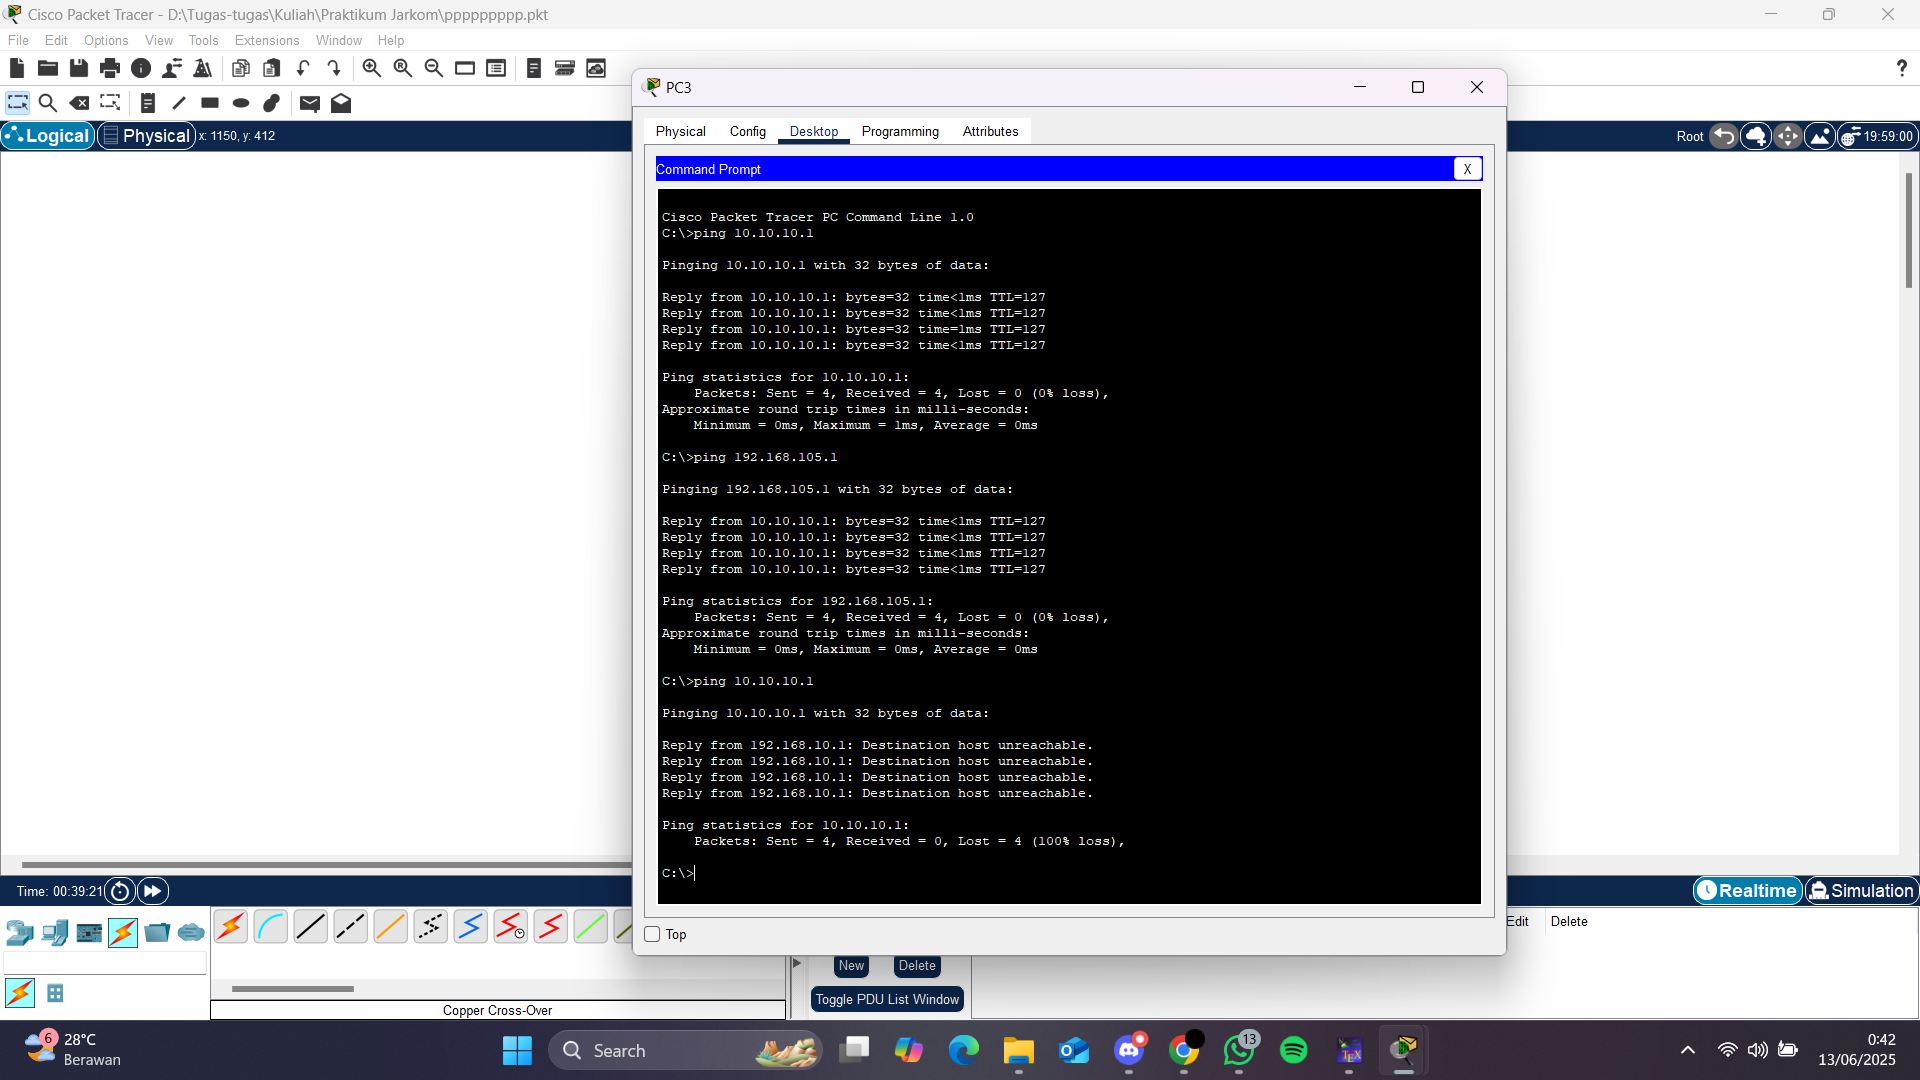
\includegraphics[width=\linewidth]{P4/img/tumod (8).png}
		\caption{Hasil ping ke server dari PC3\label{fig:konfigurasiR2}}
	\end{subfigure}
	\caption{Hasil ping ke server dari PC}
	\hspace{1cm}
\end{figure}
Untuk kasus kedua yaitu PC1 dan PC3 dilarang mengakses server dapat diterapkan dengan command sebagai berikut:
\begin{lstlisting}
	Router(config)#interface fa1/0
	Router(config-if)#ip access-list 100 in
	Router(config-if)#no ip access-list 101 in
	Router(config-if)#ip access-list 102 in
\end{lstlisting}
Command di atas akan memblokir PC1 dan PC3 saja lalu mengangkat pemblokiran PC2 (karena sebelumnya PC2 diblokir aksesnya). 
\begin{figure}[H]
	\centering
	\begin{subfigure}[b]{0.4\linewidth}
		\centering
		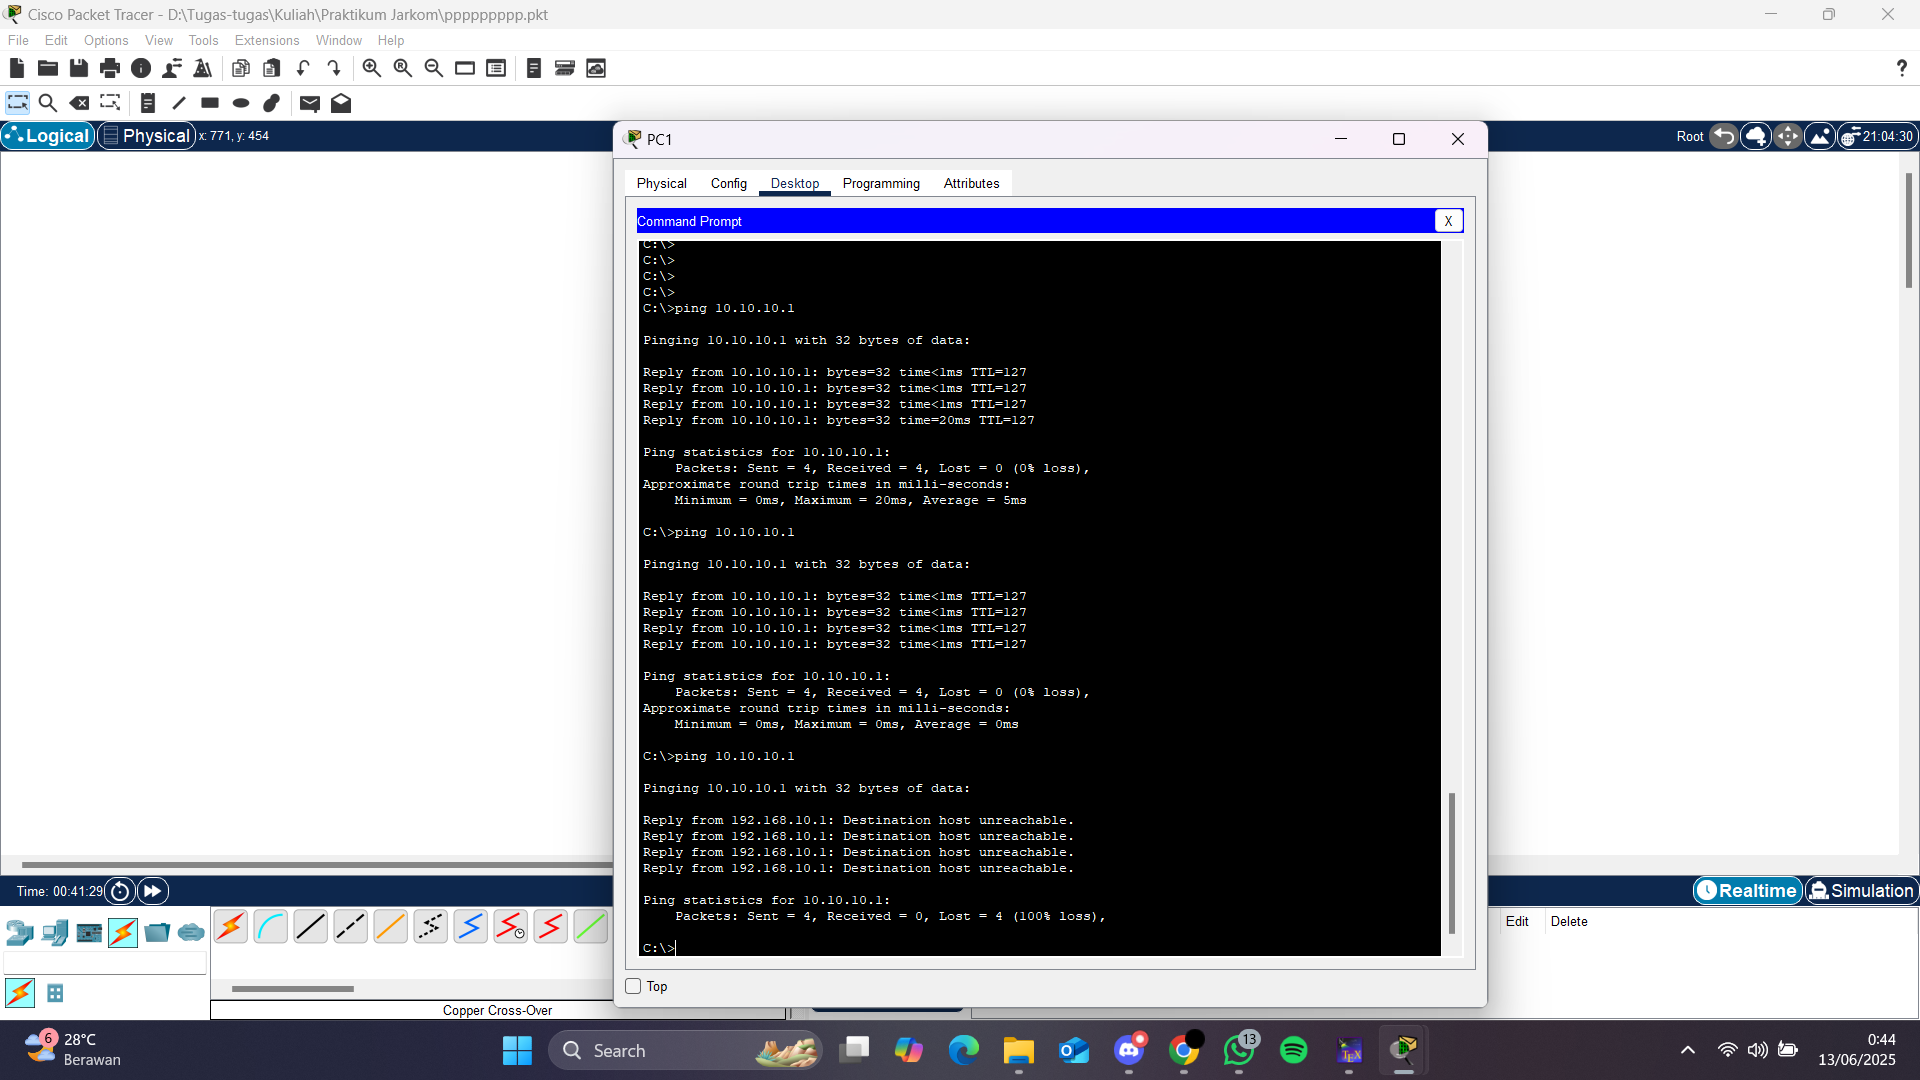
\includegraphics[width=\linewidth]{P4/img/tumod (11).png}
		\caption{Hasil ping ke server dari PC1\label{fig:konfigurasiR1}}
	\end{subfigure}
	\begin{subfigure}[b]{0.4\linewidth}
		\centering
		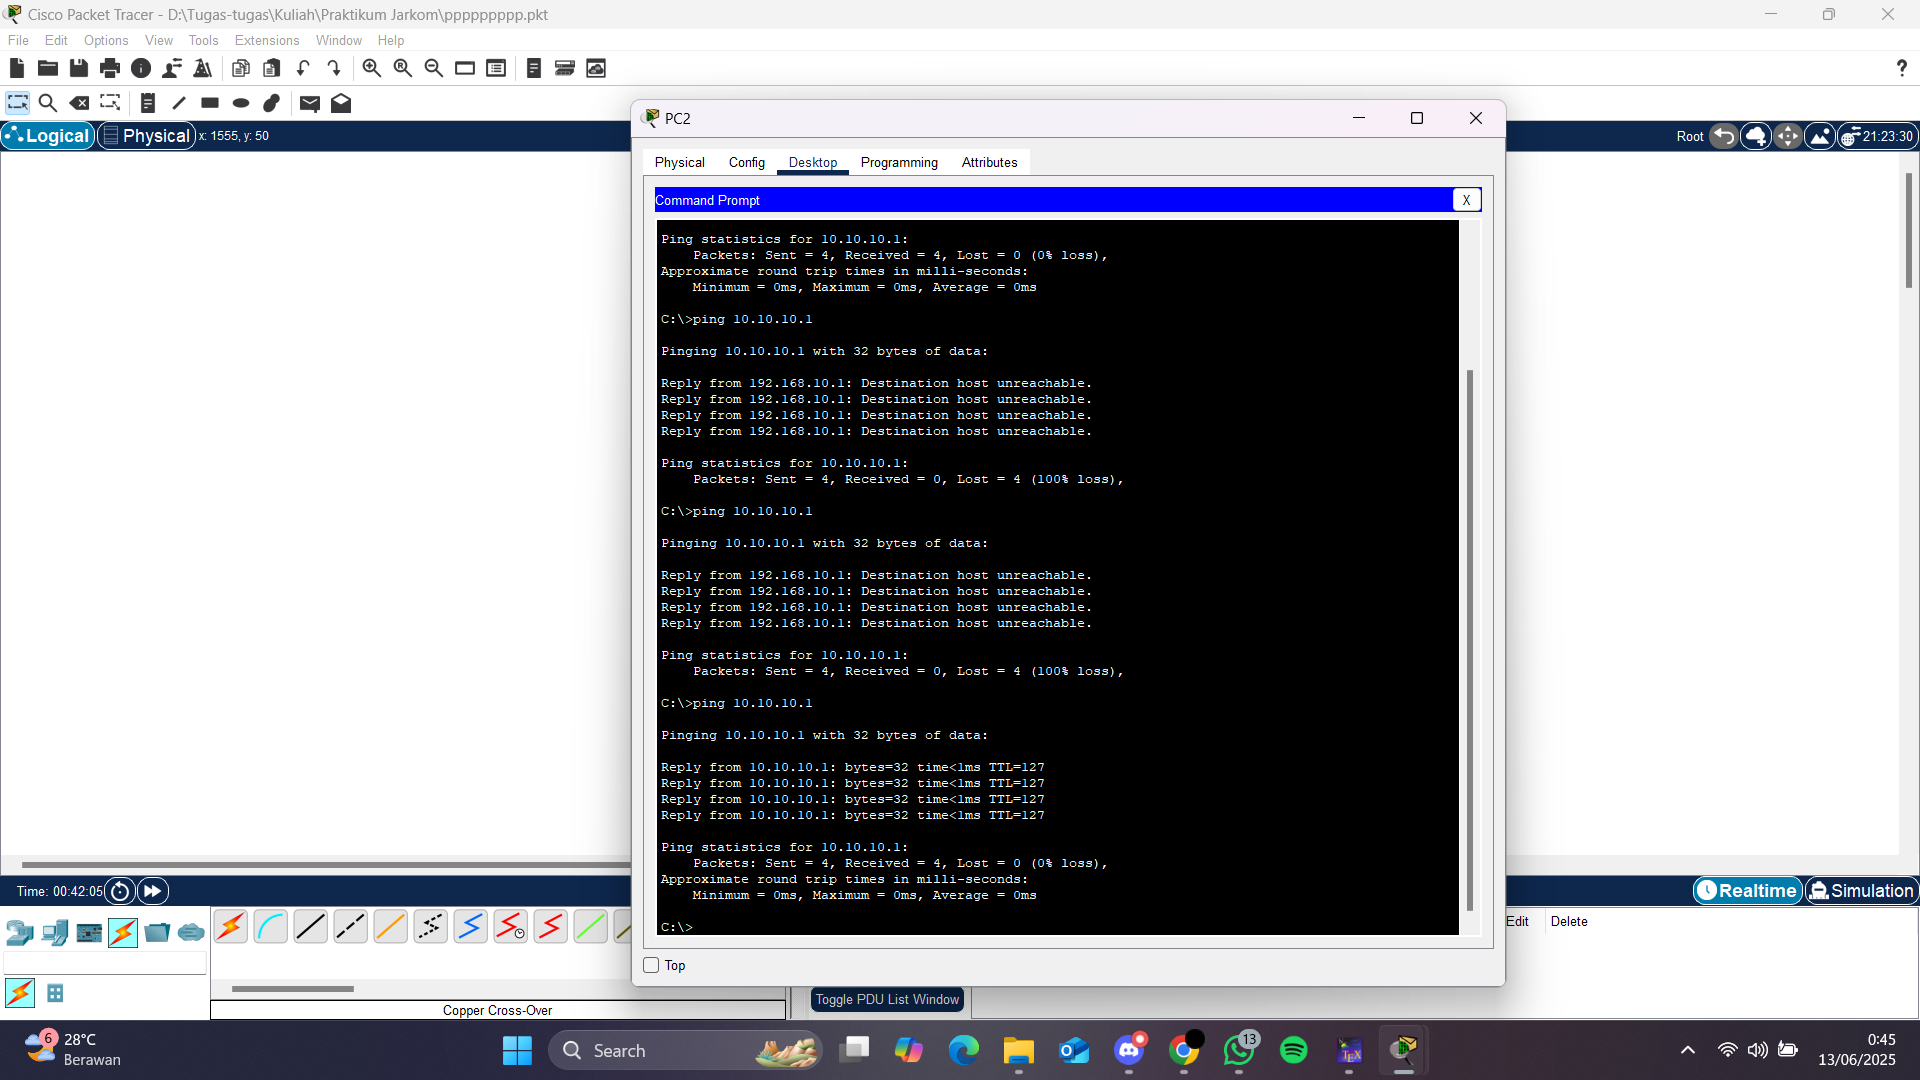
\includegraphics[width=\linewidth]{P4/img/tumod (13).png}
		\caption{Hasil ping ke server dari PC2\label{fig:konfigurasiR2}}
	\end{subfigure}
	\begin{subfigure}[b]{0.4\linewidth}
		\centering
		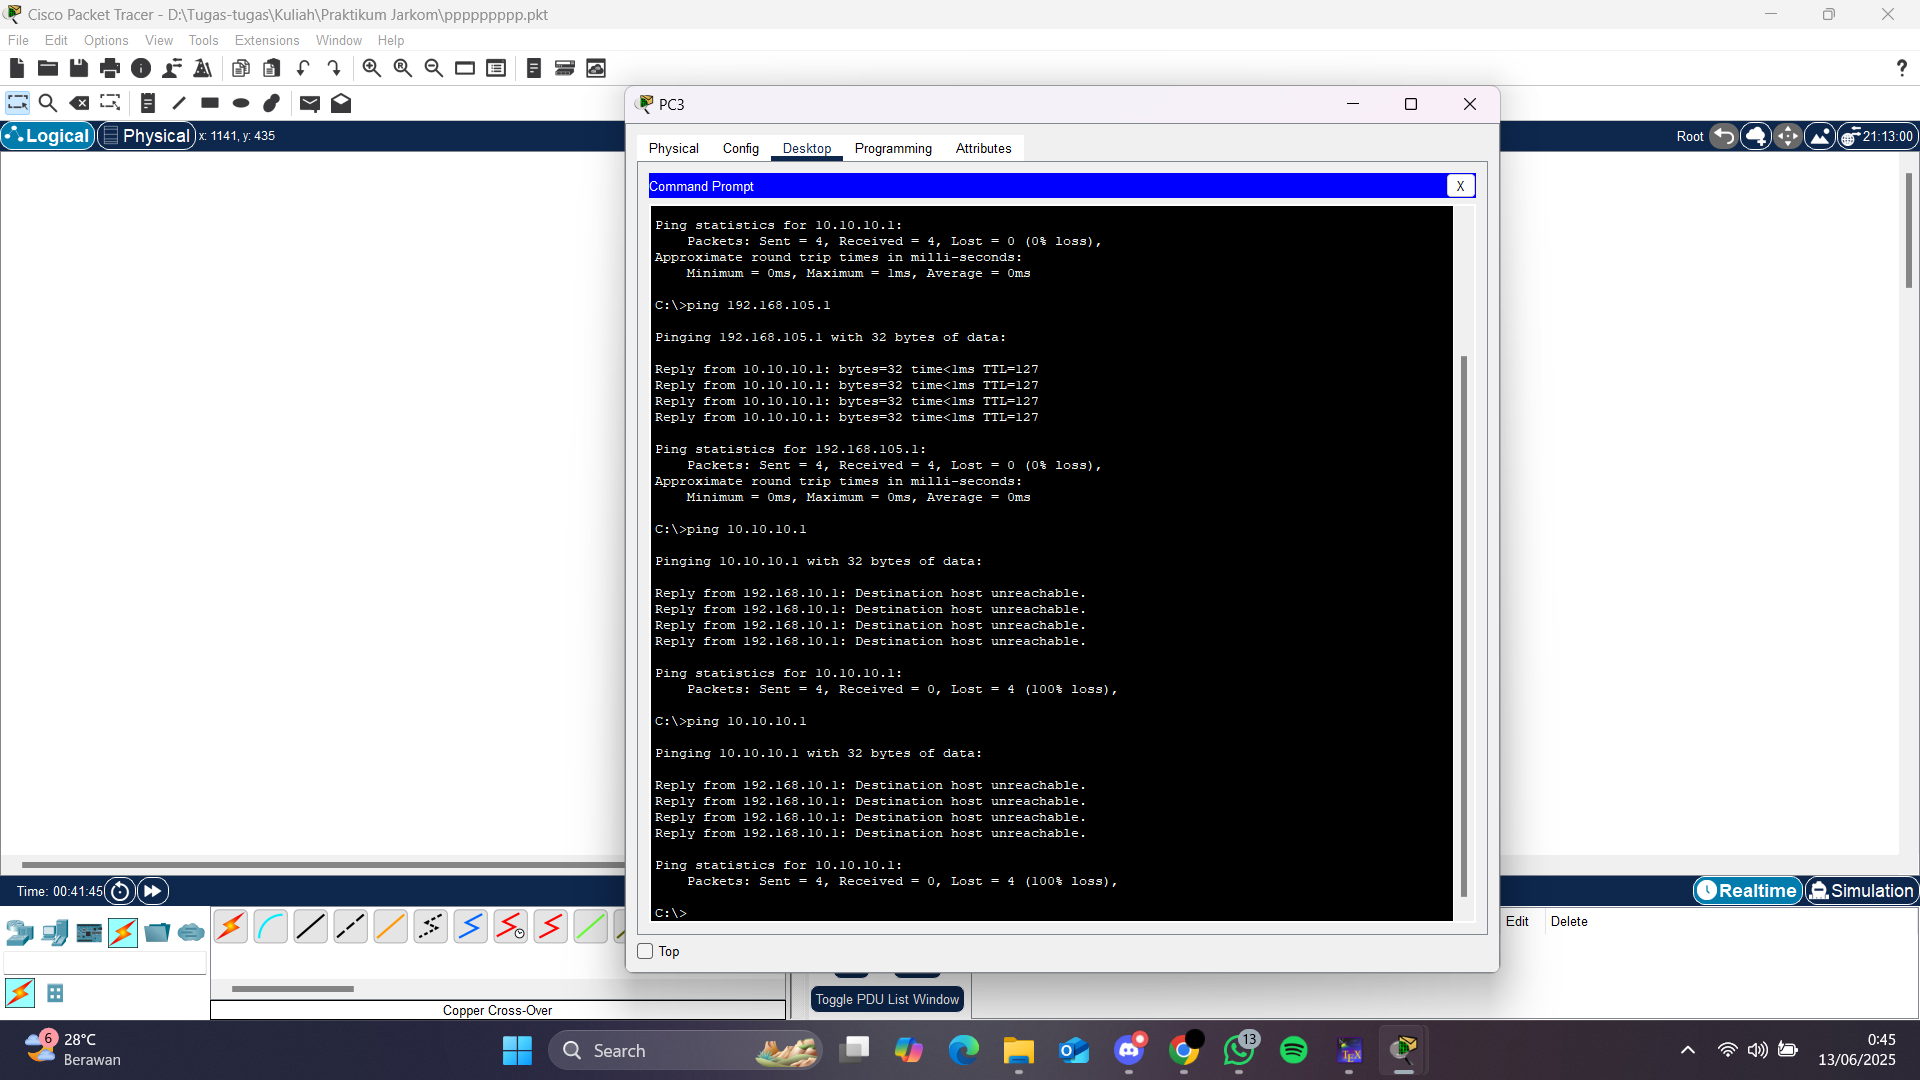
\includegraphics[width=\linewidth]{P4/img/tumod (12).png}
		\caption{Hasil ping ke server dari PC3\label{fig:konfigurasiR2}}
	\end{subfigure}
	\caption{Hasil ping ke server dari PC}
	\hspace{1cm}
\end{figure}
Dengan menerapkan access list, maka akses dari PC ke server dapat dibatasi namun tidak akan mempengaruhi komunikasi LAN antar PC sama sekali.
\section{Kesimpulan}
Adannya NAT dan firewall memungkinkan perancangan jaringan yang lebih murah (berkat kemampuan NAT untuk mentraslasikan banyak IP lokal menjadi IP publik yang lebih sedikit jumlahnya) dan lebih aman (berkat firewall yang dapat membatasi akses terhadap komunikasi dan konten). Berdasarkan hasil percobaan, baik NAT dan firewall sudah bekerja sesuai dengan teori dan hasil yang didapatkan sesuai dengan hasil yang diharapkan.

\section{Lampiran}
\subsection{Dokumentasi saat praktikum}
\begin{figure}[H]
	\centering
	\begin{subfigure}[b]{0.4\linewidth}
		\centering
		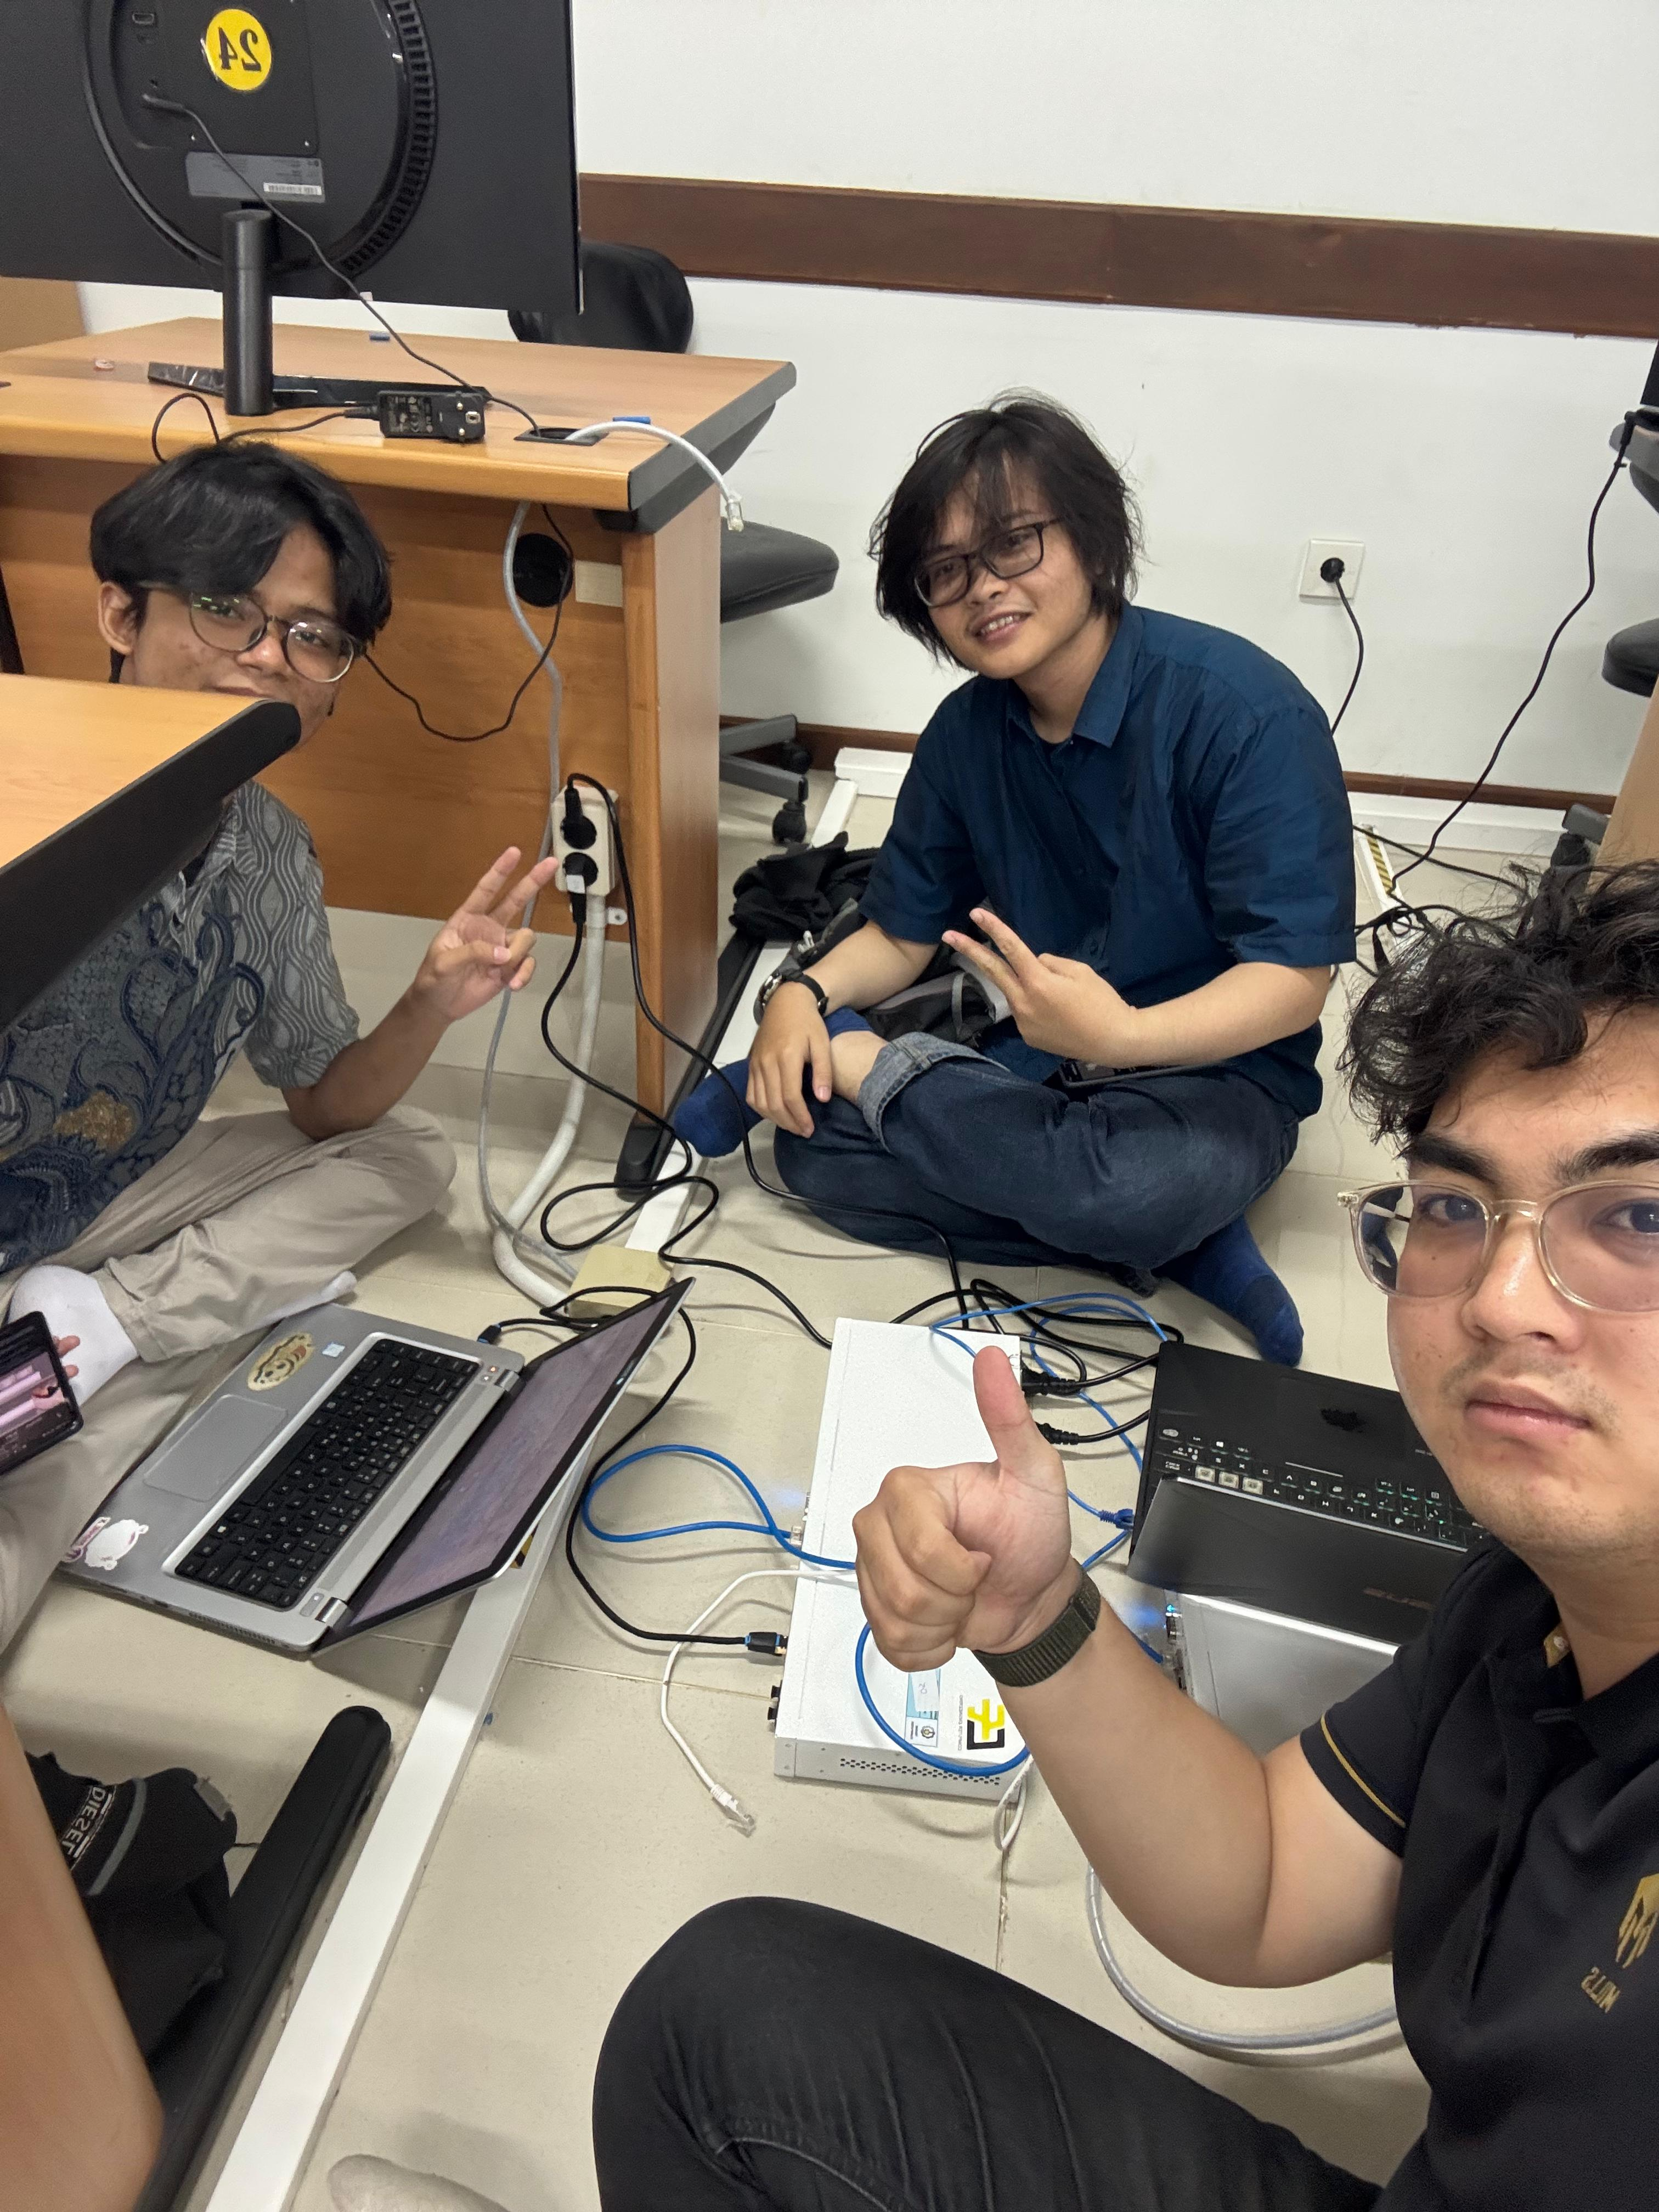
\includegraphics[width=\linewidth]{P4/img/dokum1.jpg}
	\end{subfigure}
	\begin{subfigure}[b]{0.4\linewidth}
		\centering
		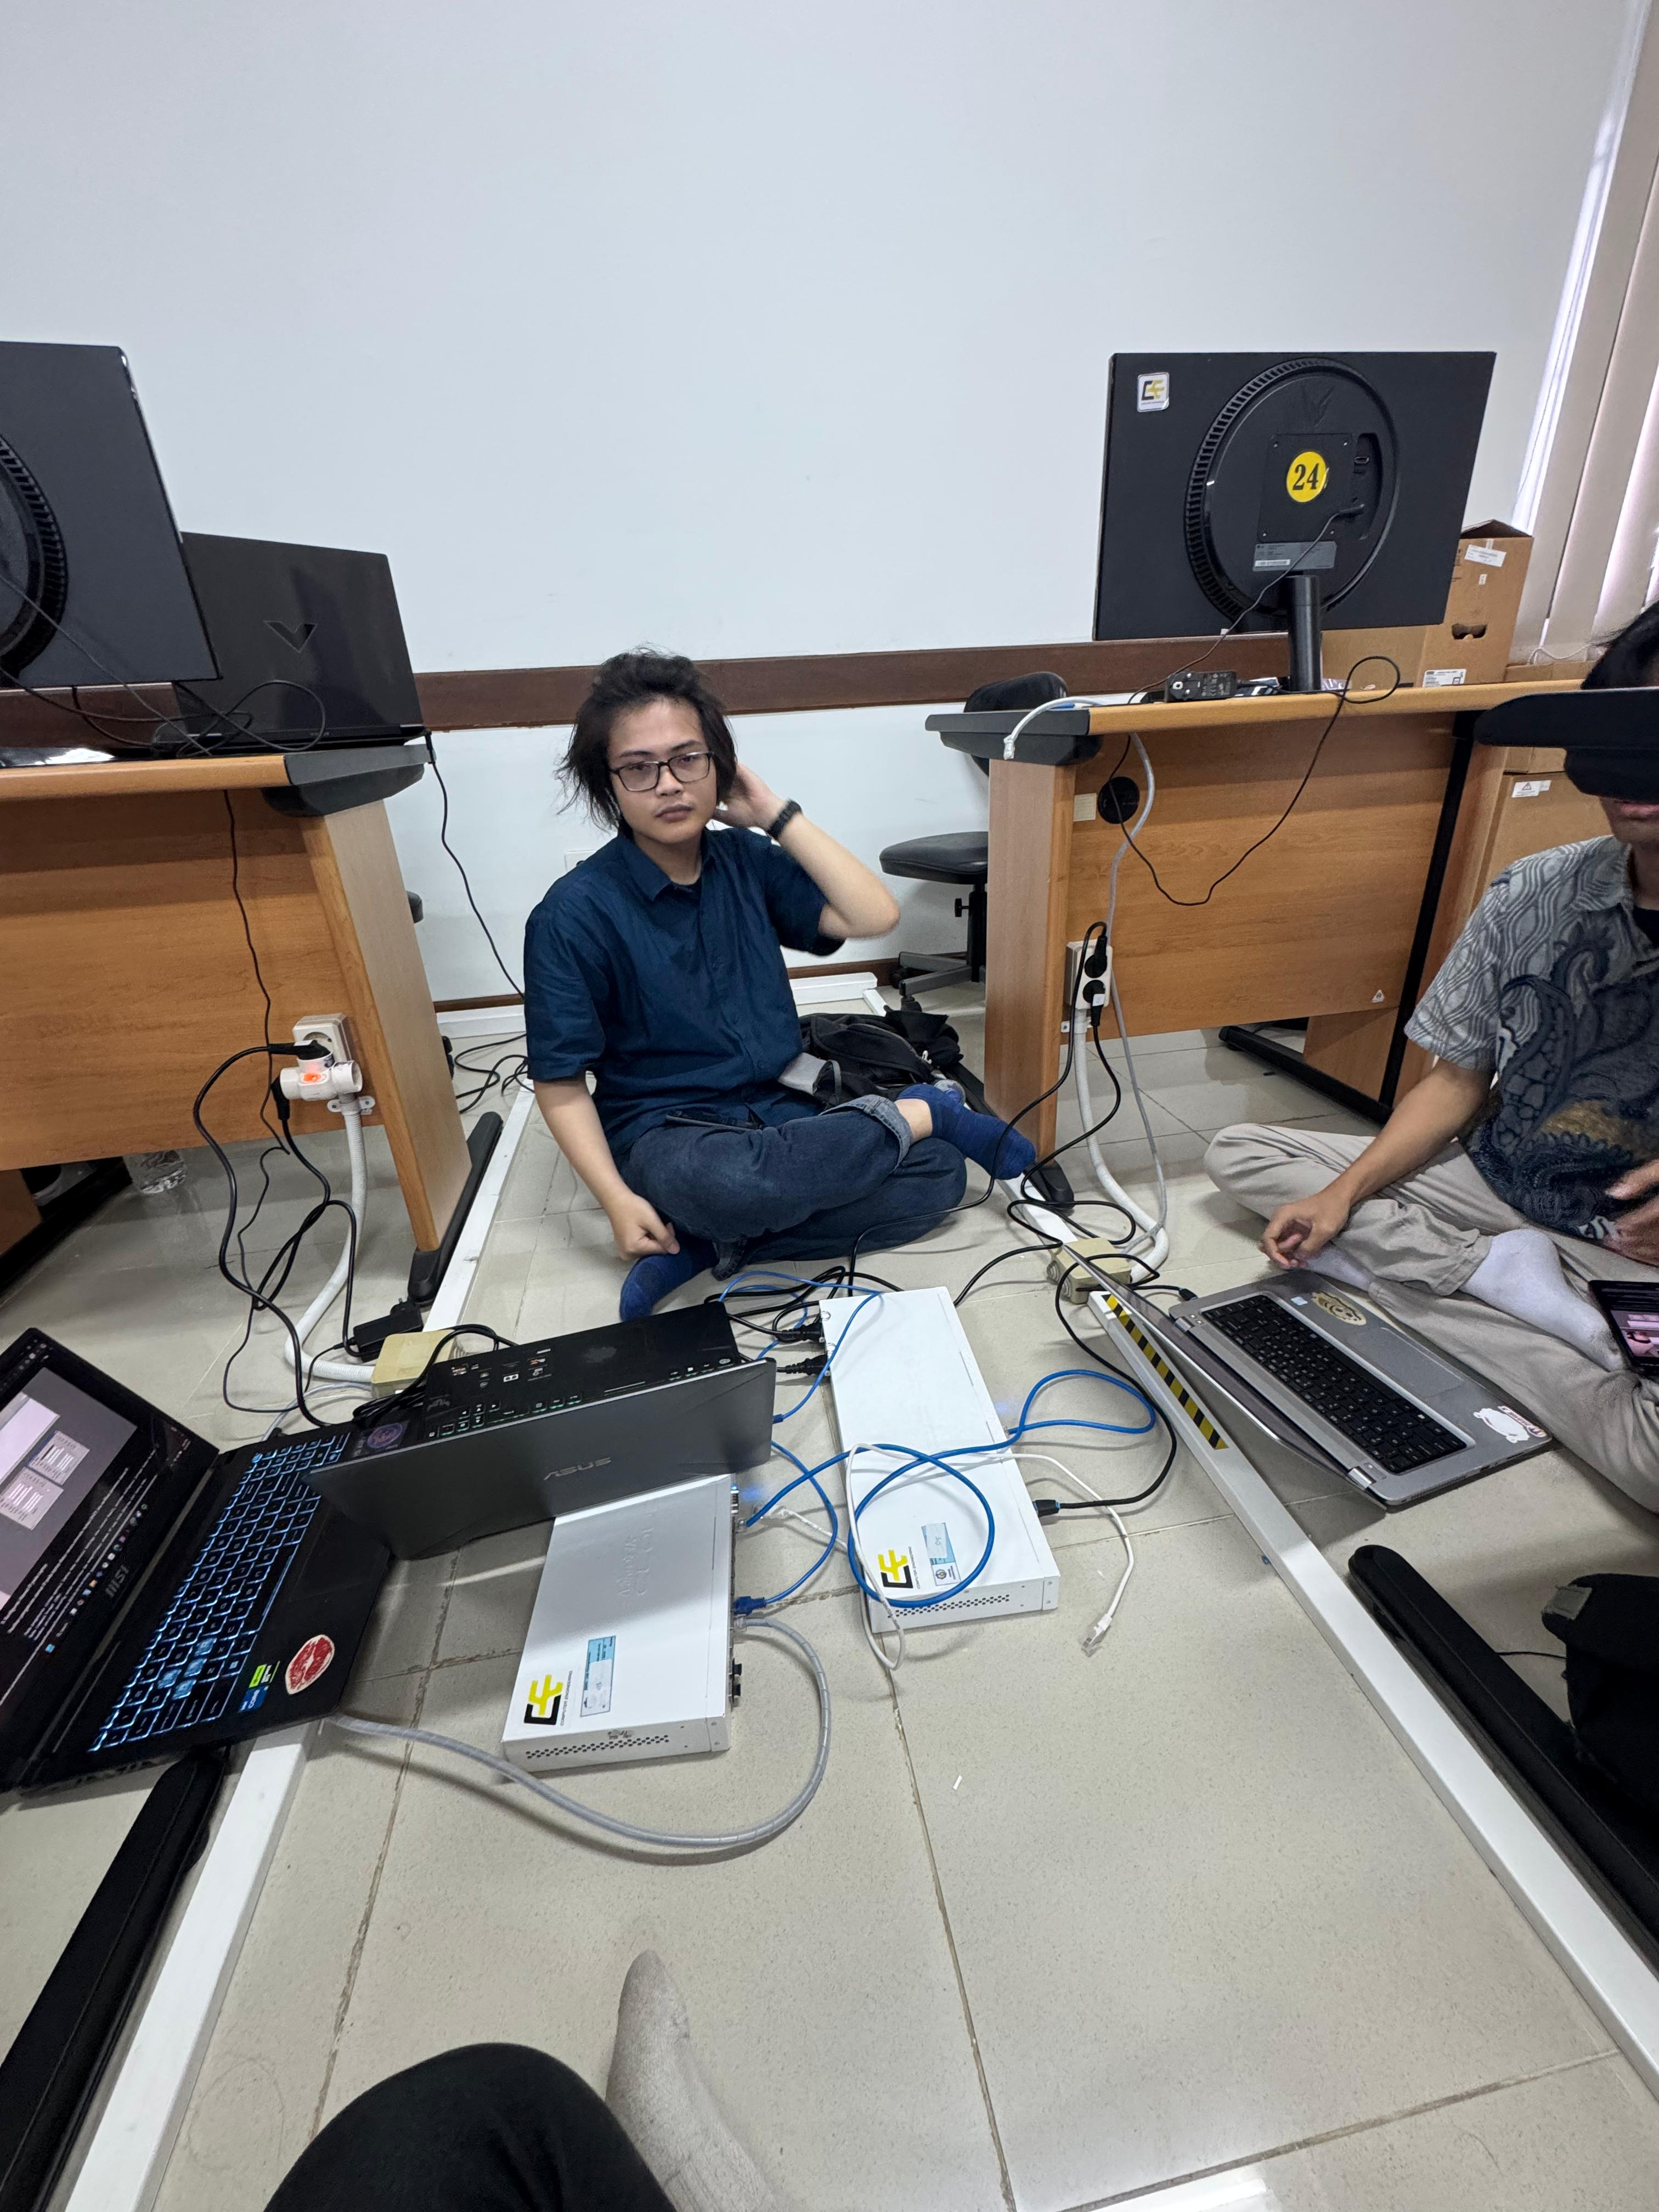
\includegraphics[width=\linewidth]{P4/img/dokum2.jpg}
	\end{subfigure}
	\caption{Dokumentasi praktikum}
	\hspace{1cm}
\end{figure}
